\begin{comment}

version 1: 	
coinciding event building; not a two single photoelectrons accidental coinciding; not a narrow pulse;  not a right triangle shape pulse; not a s1 s2 like pulse; not saturate; not a long duration pulse; not a short duration pulse; time veto 1; time veto 2 (C \& NFC \& NNRRW \& NRT \& NS1S2 \& NSat \& NL \& NS \&TV1 \&TV2).

version 2: 

coinciding event building; 
not a noise like signal; 
not a narrow signal; 
not a two single photoelectrons accidental coinciding signal; 
not a top-heavy signal; 
not a bottom-heavy signal; 
not a extremely long duration signal; 
not a right triangle shape signal; 
not a s1 s2 like signal; 
not a saturated signal; 
not a long duration signal; 
not a short duration signal; 
apply time veto selection 1;  
apply time veto selection 2;  
(C \& NNoise \&  NNRRW \& NFC \&NTH \& NBH \& NL1 \& NRT \& NS1S2 \& NSat \& NL \& NS \& TV1).
\end{comment}

\section{Signal selections}
\label{sec:cuts}
This section discusses signal selections, also known as cuts, that are used in the \gtest\ analysis. The purpose of this analysis is searching for \ees s from tested grid wires, and correctly estimating the rate of this process. For this purpose,  signal selections on different parameter spaces are carried out to identify background signals from \ees s. \todo{For each signal selection, the possibility of removing \ees is evaluated.} The primary principle of signal selections is to get a clean population of the \ees s to get a reliable estimation of its rate. Other than that, since \ees s are in most situation rare in the detector, signal selections of these \ees s are done conservatively; that is to keep as many candidates for \ees s as possible. 

An \ees\ should: 
\begin{itemize}
\item have the correct signal shape, and
\item be an uncorrelated signal from previous signals in time.
\end{itemize}

Based on the characteristics we summarized previously about \ees\ and other different signals in the detector, a list of selections are applied successively to get the clean population of the \ees s. The algorithm of each selection and the event populations each selection removes are also discussed.     

%%%%%%%%%%%%%%%%%%%%%%%%%%%%
\subsection{Signal selections based on signal shape}
Signal shape is one of the most important signature for \ees s . It includes the aspects of the signal area, the signal duration, and the \sphe\ rate at different time region during the event.
\subsubsection{coinciding found}
\label{sec:cuts coindence found}
\paragraph{Definition:}
Both PMTs have signals that occur within a time difference smaller than CWW. 
\paragraph{Purpose:}
This selection is to make sure that the signal of interest is unlikely to be from a dark current signal in one PMT, %afterpulsing in one PMT, misbehavior period of one PMT, 
or \sphe\ from other sources in one PMT (e.g. fluorescence light from PTFE, or light from discharges). 

The process of coinciding finding and coinciding event building is discussed in the data processing section in Section~\ref{par:coinbuild}. An example result from coinciding event building is shown in Fig.~\ref{fig:signal selection 03}. The signal area has a various distribution mostly in the range of \SIrange{e-1}{e5}{\phe}, when the \rpd, and the TBA, top-bottom asymmetry, are mostly distributed in the range of \SIrange{e1}{e5}{\ns} and \numrange{-1}{1}. Several ``hot spots" that are seen in the figure correspond to different activities in the detector, which will be explained later in each separate section of signal selection. Among these ``hot spots", the horizontal strap shape spot at signal area in the range of \SIrange{e1}{e2}{\phe}, \rpd\ in the range of \SIrange{e3}{e4}{\ns}, is likely to contain the potential \ees s. The locations and the counts of  different ``hot spots", including the ``hot spot" of \ees s, change as varying \opdv\ and \opgd , mainly because of the changes of the duration and the intensity of the EL process.  

Coinciding finding and coinciding event building are the fundamental part of this analysis. Signal selections defined later are based on the classification of coinciding-found signals. 

%The efficiency of this cut is \opdv\ dependent. For a proper choice of \opdv , the efficiency of this cut is larger than \SI{90}{\percent}. 
\subsubsection{Not a noise-like signal}
\paragraph{Definition:}
A coinciding-found signal has a positive signal area in all PMT channels, a higher than \num{0.5} positive to negative amplitude ratio,  and a positive \rpd .
\paragraph{Purpose:}
This selection is to make sure the signal of interest is not an electrical noise signal, which usually has a close to zero signal area, a close to unity positive to negative amplitude ratio, or a zero \rpd , as described in Section~\ref{sec:events noise}. The effect of this selection is shown in Fig.~\ref{fig:signal selection 04}. Noise-like signals, mostly at signal area in the range of \SI{<e0}{\phe}, \rpd\ in the range of \SI{<e3}{\ns}, are rejected.  

\subsubsection{Not a narrow (S1-like) signal}
\label{cuts:S1}
\paragraph{Definition:}
A coinciding-found signal has a \stw\ (time difference between the time of 25th percentile of the signal waveform and the time of 75th percentile of the signal waveform) larger than \SI{250}{\ns}, and  a \shw\ (time difference between the signal start time and the time of 50th percentile of the signal waveform) larger than \SI{320}{\ns}; in other words, the major width of the coinciding-found signal is not narrow. 
\paragraph{Purpose:}
This selection is to make sure the signal of interest is not a potential (1) Cherenkov radiation event, or (2) primary scintillation light (S1) from an external particle (e.g. a $\gamma$-ray, or a muon), as described in Sections~\ref{sec:events Cherenkov}, \ref{sec:events particle}, and \ref{sec:events muon}. The effect of this selection is shown in Fig.~\ref{fig:signal selection 05}. The narrow signals can generally be separated to two categories, corresponding to the two ``hot spots" in the figure. The first ``hot spot" at signal area in the range of \SIrange{e0}{e2}{\phe}, \rpd\ in the range of \SI{<5e1}{\ns}, may results from Cherenkov radiation events and primary scintillation light of low energy gamma radiation events. The second ``hot spot" at signal area \SIrange{e1}{e3}{\phe}, \rpd\ in the range of \SIrange{5e1}{2e2}{\ns} are likely from primary scintillation light of gamma radiation events and muon events. 

%Cherenkov radiation in PTFE material (and PMT window) are considered one of the potential sources for the extremely narrow pulses. 
%The Cherenkov radiation events originate from energy loss are the potential explanation for the extremely narrow pulses.
%Other than Cherenkov radiation , microscopic discharge that for last really short amount of time could also be the source of the extremely narrow coinciding pulses, see Section.~\ref{sec:microdischarge} discussion for microscopic discharge.  

%\paragraph{Method}
%pulse area density in the \SIrange{300}{800}{\ns} range is not low, 

\subsubsection{Not a two-\sphe\ accidental coinciding signal}
\paragraph{Definition:}
A coinciding-found signal has a signal area larger than \SI{2.5}{\phe}, and at least one PMT has a \stw\ larger than \SI{35}{\ns}, which is approximately twice the signal width of a \sphe .  
\paragraph{Purpose:}
This selection is to make sure the signal of interest is not a accidental coinciding of two \sphe s, which are likely from PMT dark current and other \sphe\ sources, as described in Section~\ref{sec:event misc}. %Sections~\ref{sec:events dark current}, \ref{sec:events PTFE fluo}, and \ref{sec:microdischarge}. 
The effect of this selection is shown in Fig.~\ref{fig:signal selection 06}. Two-\sphe\ accidental coinciding signals, mostly at signal area in the range of \SI{<2.5}{\phe}, \rpd\ in the range of up to \SI{\sim 2e3}{\ns} (this upper edge results from coinciding window width (CWW) in coinciding building), are rejected.
\begin{comment}
\paragraph{Method}
This cut is a combination with series of vetoes.
Pulse area and pulse duration are used for computing these vetoes.
A coinciding pulse is vetoed if the total pulse area is smaller than \SI{2.5}{\phe} and the pulse area in at least one of the PMTs is smaller than \SI{1.5}{\phe}. 
This choice is to compensate the \SI{\sim 30}{\percent} systematic fluctuation of PMT \sphe\ area. 
A coinciding pulse is also vetoed if the pulse duration in both PMTs are ``short". The definition of ``short" is a single pulse \ttwoseven\ smaller than \SI{80}{\ns}, and  $t_{95}$ smaller than \SI{320}{\ns}. The scatter plot of \ttwoseven\ and $t_{95}$ is shown in Fig.\ref{}.
The effect of this is shown in Fig.~\ref{}. 
\end{comment}
\begin{comment}
\begin{figure}[!p]
	\centering
	\begin{subfigure}[t]{\twofigurewidth}
		\centering
		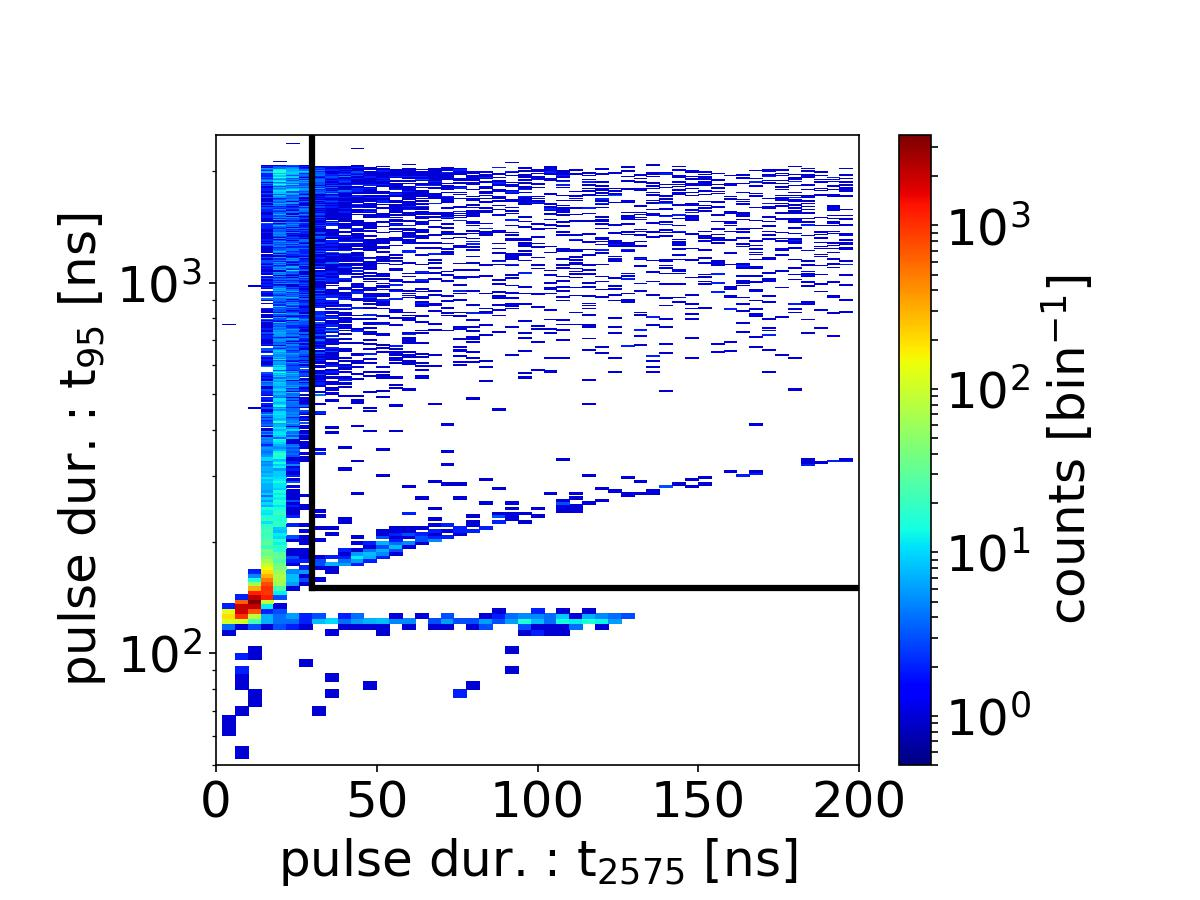
\includegraphics[width=\textwidth,clip,trim={0 0 0 0},angle=0,origin=c]{Figures/GasTest/DatasetQuality/topPMTt2575t9564767.jpg}
		\caption{}
		\label{fig:PMT t2575 t95 top}
	\end{subfigure}
	\begin{subfigure}[t]{\twofigurewidth}
		\centering
		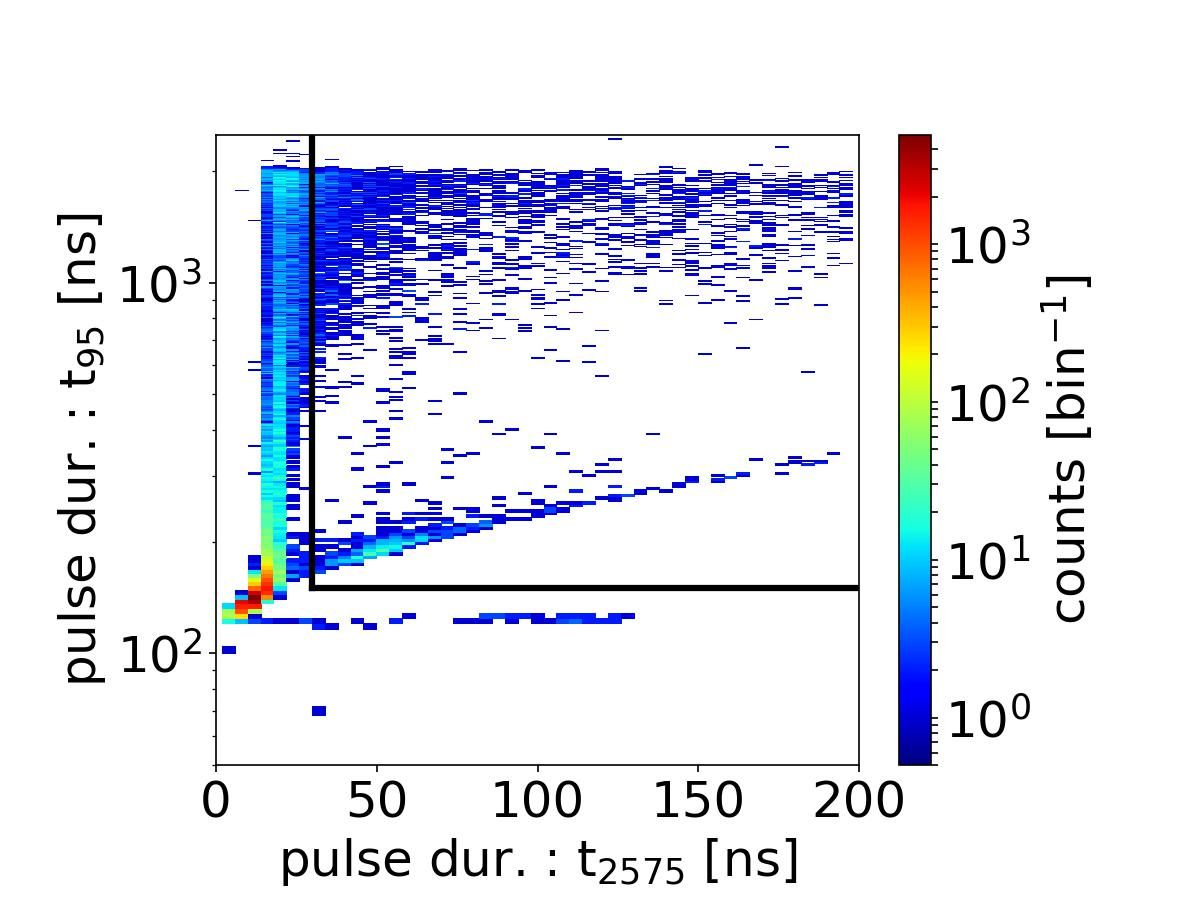
\includegraphics[width=\textwidth,clip,trim={0 0 0 0}]{Figures/GasTest/DatasetQuality/botPMTt2575t9564767.jpg}
		\caption{}
		\label{fig:PMT t2575 t95 bottom}
	\end{subfigure}
	\caption[Distribution of PMT time differences between pulses in one PMT.]{Distribution of PMT time differences between pulses in one PMT: (a) top PMT; (b) bottom PMT. }
	\label{fig:PMT t2575 t95}
\end{figure}
\end{comment}

\subsubsection{Not a top-heavy signal} %(TB_ratio:0.925 TBA: -0.0390; TB_ratio:1.005 TBA: 0.0025; TB_ratio:0.845 TBA: -0.0840; TB_ratio:1.025 TBA: 0.0123; TB_ratio:0.825 TBA: -0.0959; 
\label{sec:cuts top heavy}	
\paragraph{Definition:}
A coinciding-found signal does not have a ``top-heavy" TBA regarding its signal area. A signal-area-dependent cut on TBA is used rather than a fixed TBA value is to account for the statistically fluctuation of the TBA at low signal area region, because the counts of photons that the top and bottom PMT detected are low. 

A ``top-heavy" TBA is defined as assuming the photon counts in top PMT (T) has a binomial distribution of parameter p (success probability in a single trial) and N (number of trials), the survival function (SF) at T = $T_{\text{detected}}$ is smaller than \num{e-5}:
\begin{align}
	SF (T_{\text{detected}}) \equiv P(T > T_{\text{detected}}) = \sum_{T_{\text{detected}}}^{\infty} P (T) \d T< \num{e-5} \\
	P (T; p, N) = \binom{N}{T} p^{T} (1-p)^{N-T}
\end{align}    
where p = $B_{\text{detected}} \times$\num{1.025}/N; $T_{\text{detected}}$, $B_{\text{detected}}$ are the top and bottom PMT measured signal area in \si{phe}; and N is a sufficiently large number, chosen to be \num{e6}. A low SF($T_{\text{detected}}$) indicates a high TBA. 

\paragraph{Purpose:}
This selection is to make sure the signal of interest is not from (1)an anode cone event, (2) an anode muon cone event, (3) a PMT saturation event, or (4) a signal which misses part of the recording in the bottom PMT (likely because of PMT dead time), as described in Sections~\ref{sec:events particle anode cone}, \ref{sec:events muon anode cone}, and \ref{sec:gtest daq}. The effect of this selection is shown in Fig.~\ref{fig:signal selection 07}. The four categories of background events correspond to the four ``hot spots" in the figure. 

The ``hot spot" at signal area in the range of \SIrange{e2}{e3}{\phe}, \rpd\ in the range of \SIrange{\sim e3}{e4}{\ns}, and TBA \num{\sim 0.3}, results from EL light in the anode cone gamma radiation events. This ``hot spot" is a combination of two smaller ``hot spots". The ``hot spot" on the left (signal area \SI{\sim 2 e2}{\phe}, \rpd\ \SI{\sim 2 e3}{\ns}, and TBA \num{\sim 0.3}) may result from xenon X-rays events with typical energy of \SI{33}{\keV} in the anode cone . A xenon X-ray event in average can create \num{\sim 1.5e3} drifted electrons,\footnote{The average energy to create an electron-ion pair in xenon gas ($W_\text{ion}$) is \SI{22}{\eV} for a gamma particle, estimated from $W_\text{ion}$ for an alpha particle and a beta particle in Ref.~\cite{Fano1963, Ahlen1980, Alvarez2013}.} which produce EL light in the high electric field region around the anodic grid wires. The ``hot spot" on the right corresponds to other higher energy gamma radiation.

The location of this ``hot spot"  in the figure moves as varying \opdv . As \opdv\ increases, the electric field strength around the anodic grid wires also increases, which causes higher quantity of EL light production and signal area. At a low \opdv , the small area signals cannot be rejected by this selection. Therefore, another signal selection based on the time correlation between the signal of primary scintillation and the signal of EL of these events, is carried out, as described later in Section~\ref{sec:uncor}.

The ``hot spot" at signal area \SI{\sim e4}{\phe}, \rpd\ \SI{\sim e4}{\ns}, results from EL light in the anode cone muon events. Similar to anode cone event from gamma radiation, these events also produce free drifted electrons, which produce EL light in the high elelctric field region around the anodic grid wires. The duration of these muon events are much longer than that of gamma events is because the longer ionization track of a muon event causes the drifted electrons created in the muon event arrive the anodic grid and produce EL light in a wider time span, as described in Section~\ref{sec:events muon anode cone}. The location of this ``hot spot"  in the figure moves to high signal area as increasing \opdv . Therefore, the same argument holds for the signal selection based on the time correlation is used to reject these signals. 

The ``hot spot" strap at signal area \SI{\sim e4}{\phe}, \rpd\ \SI{\sim e3}{\ns}, and TBA \num{\sim 0.1} results from high energy particle and muon events which saturate the DAQ. Because the average \sphe\ amplitude in the bottom PMT is higher, it exceeds the upper limit of the DAQ dynamic range at a smaller counts of \sphe\ than the top PMT. Therefore, the reconstructed signal area in the bottom PMT is lower after it reaches the DAQ saturation limit, which leads to a higher signal TBA because of this DAQ saturation issue.

The ``hot spot" at TBA \num{\sim 1} results from missing part of the recording in the bottom PMT ,which is most likely because of PMT dead time. In these signals, the top PMT records the full event, when the bottom PMT only records the beginning or the end of the event. This results in a close to unity signal TBA.

\subsubsection{Not a bottom-heavy signal}
\paragraph{Definition:}
A coinciding-found signal does not have a ``bottom-heavy" TBA regarding its signal area. 

Similar to the ``top-heavy" TBA, a ``bottom-heavy" TBA is defined as assuming the photon counts in bottom PMT (B) has a binomial distribution of parameter p (success probability in a single trial) and N (number of trials), the survival function (SF) at B = $B_{\text{detected}}$ is smaller than \num{e-5}:
\begin{align}
SF (B_{\text{detected}}) \equiv P(B > B_{\text{detected}}) = \sum_{B_{\text{detected}}}^{\infty} P (B) \d B< \num{e-5} \\
P (B; p, N) = \binom{N}{B} p^{B} (1-p)^{N-B}
\end{align}    
where p = $T_{\text{detected}}$/\num{0.825}/N; $T_{\text{detected}}$, $B_{\text{detected}}$ are the top and bottom PMT measured signal area in \si{phe}; and N is a sufficiently large number, chosen to be \num{e6}. A low SF($B_{\text{detected}}$) indicates a low TBA. 
\paragraph{Purpose:}
This selection is to make sure the signal of interest is not a signal which misses part of the recording in the top PMT (likely because of PMT dead time), as described in Section~\ref{sec:gtest daq}, which is similar to the situation described in Section~\ref{sec:cuts top heavy}.

The effect of this selection is shown in Fig.~\ref{fig:signal selection 08}. Signals with TBA close to -1 are rejected because they are likely to be a signal missing part of the recording in the top PMT.

In reverse polarity operation when the top grid is cathodic and the bottom grid is anodic, the roles of ``top-heavy" and ``bottom-heavy" signal selections switches from normal polarity operation.

\subsubsection{Not a extremely long duration signal}
\paragraph{Definition:}
A coinciding-found signal has a \pud\ 1.5 times longer than the predicted EL duration from the estimated average EL region electric field and Eqn.~\ref{eqn:xenon electron drift velocity}. 
\paragraph{Purpose:}
This selection is to make sure the signal of interest is not a muon event or a multiple scatter event, as described in Sections~\ref{sec:events muon} and \ref{sec:events particle multiple scatter}. The effect of this selection is shown in Fig.~\ref{fig:signal selection 09}. The ``hot spot" at signal area \SI{\sim e4}{\phe}, \rpd\ \SI{\sim3 e3}{\ns}, and TBA \num{\sim 0} results from EL region muon events. 

\subsubsection{Not a right-angle triangle shape signal}
\todo{may be remove this cut.}
\paragraph{Definition:}
A coinciding-found signal does not have a large skewness of signal waveform and a higher photon rate at the beginning of the signal than that at the end of the signal. 

The skewness statistics of a \ees\ waveform is close to zero because the shape is close to a uniform distribution, when the skewness of a right-angle triangle shape is \num{\sim 0.96}. Therefore, this statistics is used to distinguish the right-angle triangle waveform. The skewness statistics between 5th percentile time and 95th percentile time (skew$_\text{05-95}$) and the skewness statistics between 15th percentile time and 85th percentile time (skew$_\text{15-85}$) are used to effect from the outlier. A large skewness is defined as skew$_\text{05-95}$ \num{>0.2} and skew$_\text{15-85}$ \num{>0.1}.

Since the skewness statistics are sometimes effected by outlier, another method is carried out based on comparing the photon rate the beginning of the signal and that at the end of the signal as a supplement. A higher photon rate at region A than region B is defined below. The detected signal area and duration of region A and region B is noted as $A_{\text{detected}}$,  $B_{\text{detected}}$, $t_{A}$,  $t_{B}$. Assuming the photon counts in region A in a simulation ($A_{\text{sim}}$) has a binomial distribution of parameter p (success probability in a single trial) and N (number of trials), the survival function (SF) at $A_{\text{sim}}$ = $A_{\text{detected}}$ is smaller than \num{e-6}:
\begin{align}
SF (A_{\text{detected}}) \equiv P(A_{\text{sim}} > A_{\text{detected}}) = \sum_{A_{\text{detected}}}^{\infty} P (A) \d A< \num{e-6} \\
P (A; p, N) = \binom{N}{A} p^{A} (1-p)^{N-A}
\end{align}    
where p = \num{1.2} $\times B_{\text{detected}} \times t_{A}/t_{B}$/N; and N is a sufficiently large number, chosen to be \num{e6}. A low SF ($A_{\text{detected}}$) indicates a higher photon rate at region A than region B. If the photon rate between the 5th and 15th time percentiles, or between 300 and 800 ns after the recording start time of the event, is higher than that between the 50th and 80th time percentiles, we say that the signal has a higher photon rate at the beginning than at the end.

\paragraph{Purpose:}
This selection is to make sure the signal of interest is not a EL region muon event, or a S1 S2 event in the EL region, as described in Sections~\ref{sec:events muon EL region} and \ref{sec:events particle EL region}. The muon events happening between the grid rings has a lower light production and light collection than those happing between the grid wires. These grid-ring-region events usually does have a ``long tail" in the signal because the muon track does not pass the anode region creating free drifted electrons. These two reasons make it hard to distinguish muon events happening between the grid rings by a long signal duration or a large signal area as that between the grid wires. The effect of this selection is shown in Fig.~\ref{fig:signal selection 10}. Therefore, this selection is used.

\subsubsection{Not an S1 S2 like signal}
\todo{may be remove this cut.}
\paragraph{Definition:}
A coinciding-found signal does not have a low photon rate in the range of \SIrange{300}{800}{\ns} since the recording start time of the signal. 

Since in this type of events, the photon rate is low between the S1 and S2 signal, we compare the photon rate in the time region immediately after S1 to other time region to distinguish these events. An S1 signal usually lasts less than \SI{180}{\ns}, therefore ending \SI{300}{\ns} after the recording start time of the signal, because of the pre-delay recording described in Sections~\ref{sec:gtest daq} and \ref{sec:gtest data process}. The compared region are between \SI{800}{\ns} since the recording start time of the signal and 90th percentile time, between 25th percentile time and 90th percentile time, between 50th percentile time and 75th percentile time, and between 50th percentile time and 95th percentile time.

\paragraph{Purpose:}
This selection is to make sure the signal of interest is not from an S1 S2 event in the cathode corner, as described in Section~\ref{sec:events particle EL region}. The effect of this selection is shown in Fig.~\ref{fig:signal selection 11}.

\subsubsection{Not a saturated signal}
\paragraph{Definition:}
A coinciding-found signal does not have any PMT saturated.
\paragraph{Purpose:}
This selection is to make sure the signal of interest is not from a particle or muon event that have large signal area, unlike \ees\ which usually does not produce large signal that saturate any PMT. The effect of this selection is shown in Fig.~\ref{fig:signal selection 12}.

\subsubsection{Not a long duration signal}
\paragraph{Definition:}
A coinciding-found signal has a \rpd\ 1.5 times longer than the predicted \ees\ \rpd\ from the estimated average EL region electric field and Eqn.~\ref{eqn:xenon electron drift velocity}. 
\paragraph{Purpose:}
This selection is to make sure the signal of interest is not a muon event or a multiple scatter event, as described in Sections~\ref{sec:events muon} and \ref{sec:events particle multiple scatter}. The effect of this selection is shown in Fig.~\ref{fig:signal selection 13}. 

\subsubsection{Not a short duration signal}
\paragraph{Definition:}
A coinciding-found signal has a \rpd\ shorter than 0.64 times the predicted \ees\ duration from the estimated average EL region electric field and Eqn.~\ref{eqn:xenon electron drift velocity}, and shorter than 5 sigma from the predicted \ees\ \rpd\ duration. 
\paragraph{Purpose:}
This selection is to make sure the signal of interest is not a grid ring region event (likely originating from muon or particle), as described in Sections~\ref{sec:events muon EL region} and \ref{sec:events particle EL region}. The effect of this selection is shown in Fig.~\ref{fig:signal selection 14}. An event happening in the grid ring region has low light collection efficiency and is therefore hard to be distinguished by its shape. However, it usually has a shorter duration, and can therefore be rejected by this selection.

%%%%%%%%%%%%%%%%%%%%%%%%%%%%
\subsection{Signal selections based on previous signals}
\label{sec:uncor}
Previous signals may correlate with the later signals. There are two major types of correlation signals.  One type of correlation signals is between primary scintillation light and EL light from the ionization electrons. In an anode cone region event, primary scintillation light are produced immediately after a particle interaction, when the ionization electrons take time to drift to the anodic grid to produce EL light, as described in Sections~\ref{sec:events particle anode cone} and \ref{sec:events muon anode cone}. Therefore, we can the correlation between primary scintillation light and EL light to determine these events. The second type of correlation signals is fluorescence signals succeeding large-area signals, as described in Section~\ref{sec:events PTFE fluo}. Since the fluorescence signals may look like \ees s, the correlation between the fluorescence signals and the large-area signals is the only method to distinguish these fluorescence signals. Therefore, we use signal selections based on the previous signal area to reject these background events.

Moreover, previous signals also introduce PMT dead time issue, as described in Section~\ref{sec:gtest daq}. PMT dead time issue causes an incomplete recording of the signals immediately following another signal. To address this issue, we subtract a segment of time after each recorded pulse from the live time of study and eliminate all signals that is recorded in this time period. Therefore, we use signal selections based on the previous signal duration to reject these background events.

These two signal selections previously mentioned may veto good candidate \ees s . Therefore, the survival ratio of the candidate \ees s from these signal selection need to be estimated.

%This cut also removes \todo{describe the small area stuff.}
%This cut also resolves the dead time issue, \todo{explain here.}
%This selection is to make sure the signal of interest is not a part of anode cone event. This is also to resolve dead time of DAQ. 

\subsubsection{Previous signal area veto}
\paragraph{Definition:}
A coinciding-found signal (1) is not following another pulse in any PMT with pulse area larger than \SI{3.5}{\phe} within \SI{150}{\us}, (2) is not following another pulse in any PMT with pulse area larger than \SI{e3}{\phe} within \SI{300}{\us}, and (3) is not following another pulse in any PMT with pulse area larger than \SI{e4}{\phe} within \SI{1000}{\us}.
\paragraph{Purpose:}
The 150-us veto is to make sure that the signal of interest is not the EL light from an anode cone region event, as described in Sections~\ref{sec:events particle anode cone} and \ref{sec:events muon anode cone}. Primary scintillation light signals and EL signals are related in time in anode cone region events.  Therefore, this veto can reject the anode cone region event EL signal which usually happens after the primary scintillation light signals. The time difference between the two signals is the time that takes ionization electrons to drift to the anodic grid, which is smaller than \SI{150}{\us} for \opva\ larger than \SI{3}{\kV}. Primary scintillation light signals mostly have their pulse area larger than \SI{3}{\phe} in at least one PMT, which drives the choice of pulse area value for this selection.

The 200-us veto and the 1000-us veto are to make sure that the signal of interest is not fluorescence signals succeeding large-area signals, as described in Section~\ref{sec:events PTFE fluo}. With the segment of time cut off, the fluorescence induced \sphe\ rate is below \SI{e4}{\Hz}, therefore the rate of accidental coinciding with more than \SI{3}{\phe} is below \SI{4}{\Hz} for the chosen CWW. 

The effect of this selection is shown in Fig.~\ref{fig:signal selection 15}. Even though not shown in this figure, this selection is also effective in removing the ``hot spot" at signal area in the range of \SIrange{e2}{e3}{\phe}, \rpd\ in the range of \SIrange{\sim e3}{e4}{\ns}, and TBA \num{\sim 0.3}, resulting from EL light in the anode cone gamma radiation events, which is shown in Fig.~\ref{fig:signal selection 07}. This selection is necessary when \opdv\ is small because the signal selection based on TBA is less effective in such \opdv , as discussed in Section~\ref{sec:cuts top heavy} . 
%Source of this type of background are: (1) an anode region event, and (2) fluorescence photons following a signal with large signal area. The cuts for resolving these two backgrounds are (1) short following period veto, and (2) long following period veto.
%Signal shape is one of the most important signature for \ees s . It includes the aspects of the signal area, the signal duration, and the \sphe\ rate at different time region during the event.

\subsubsection{Previous signal duration veto}
\paragraph{Definition:}
A coinciding-found signal (1) is not following another pulse in any PMT within \SI{10}{\us}, (2) is not following another pulse in any PMT with pulse duration longer than \SI{3}{\us} within \SI{20}{\us}, (3) is not following another pulse in any PMT with pulse duration longer than \SI{10}{\us} within \SI{40}{\us}, and (4) is not following another pulse in any PMT with pulse duration longer than \SI{30}{\us} within \SI{200}{\us}.
\paragraph{Purpose:}
This selection is to make sure the PMT dead time issue is addressed. The effect of this selection is shown in Fig.~\ref{fig:signal selection 16}. Since this selection overlaps with other selections applied previously, in this particular example figure, few events are removed by this selection.
%The rate of PTFE fluorescence is strongly dependent on the previous luminance history in the detector.
%This cut overlaps with the short following period veto cut.   

\begin{landscape}
	
\begin{figure}[!p]
	\centering
	\begin{subfigure}[t]{0.32\textwidth} %0.44\textwidth is the maximum to fit three column in a row
		\centering
		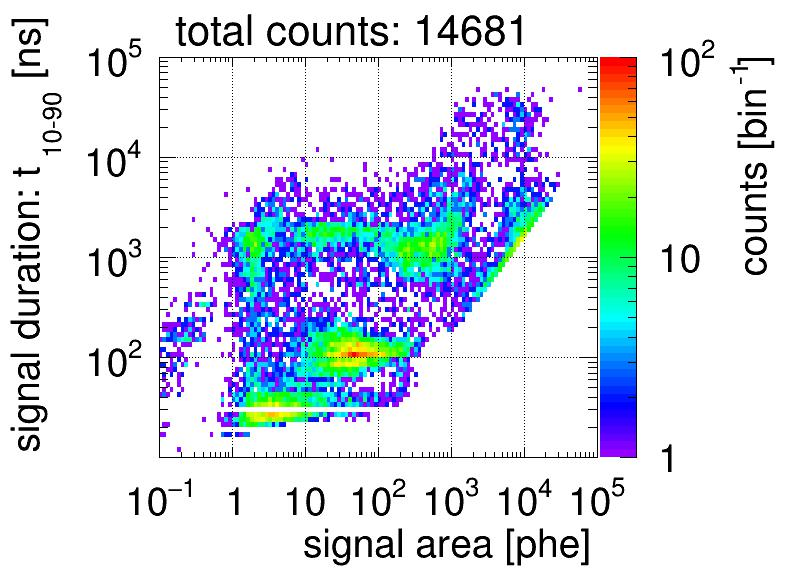
\includegraphics[width=\figurewidth,clip,trim={0 98 0 15}]{Figures/GasTest/CutsValid/res64767/pdpa03Vecfig64767.jpg}
		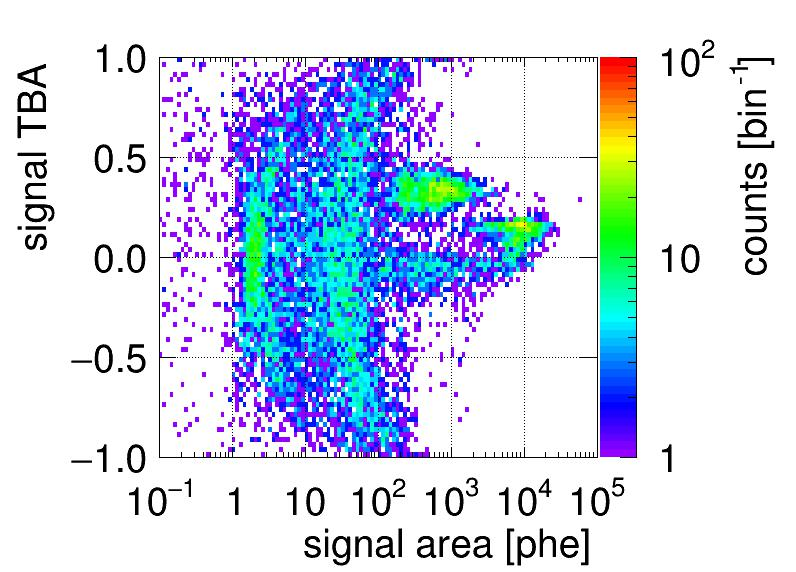
\includegraphics[width=\figurewidth,clip,trim={0 8 0 40}]{Figures/GasTest/CutsValid/res64767/tbapa03Vecfig64767.jpg}
%		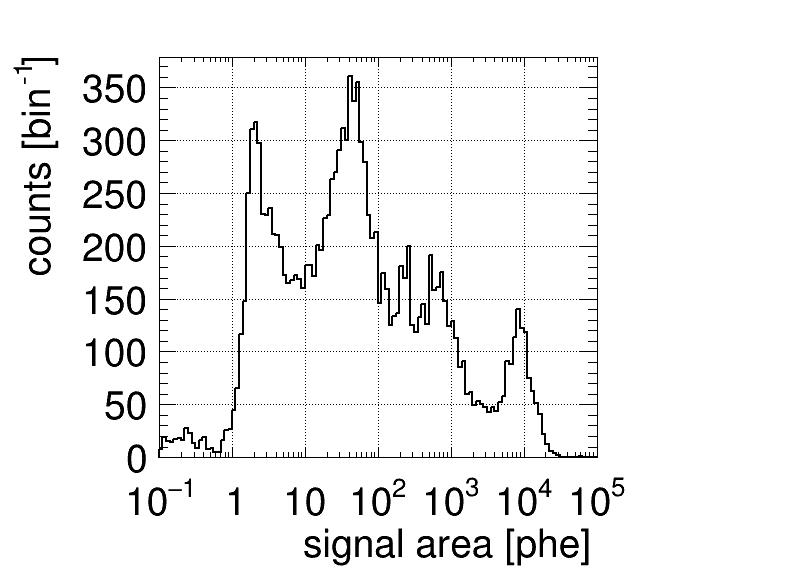
\includegraphics[width=\figurewidth,clip,trim={0 0 0 0}]{Figures/GasTest/CutsValid/res64767/pa03Vecfig64767.jpg}
		\caption{}
		\label{fig:signal selection 03}
	\end{subfigure}
	\begin{subfigure}[t]{0.32\textwidth}
		\centering
		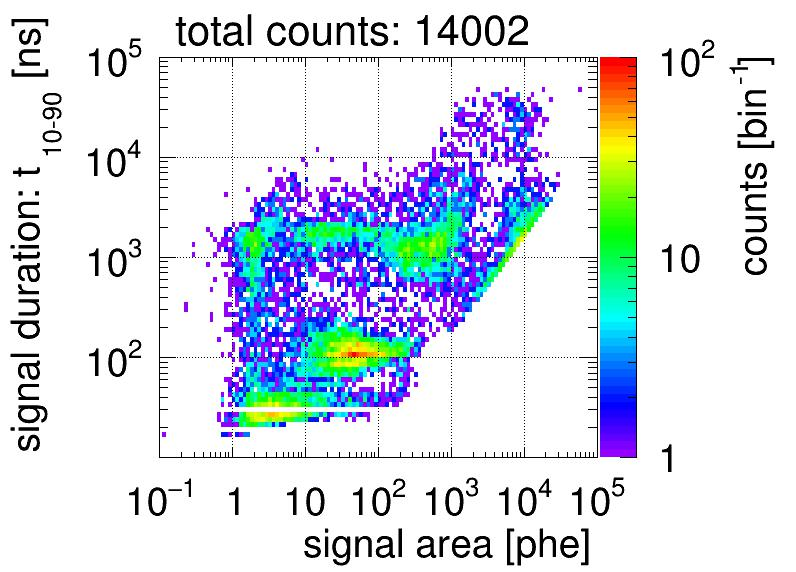
\includegraphics[width=\figurewidth,clip,trim={0 98 0 15}]{Figures/GasTest/CutsValid/res64767/pdpa04Vecfig64767.jpg}
		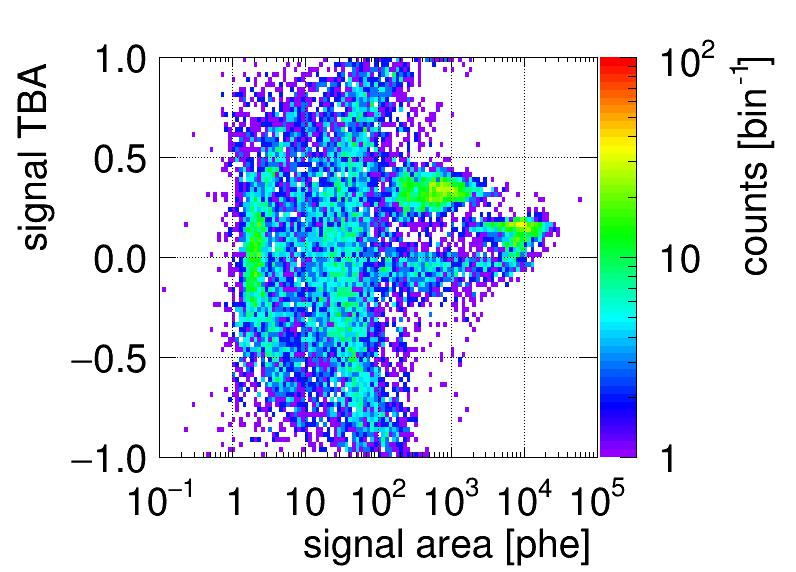
\includegraphics[width=\figurewidth,clip,trim={0 98 0 40}]{Figures/GasTest/CutsValid/res64767/tbapa04Vecfig64767.jpg}
		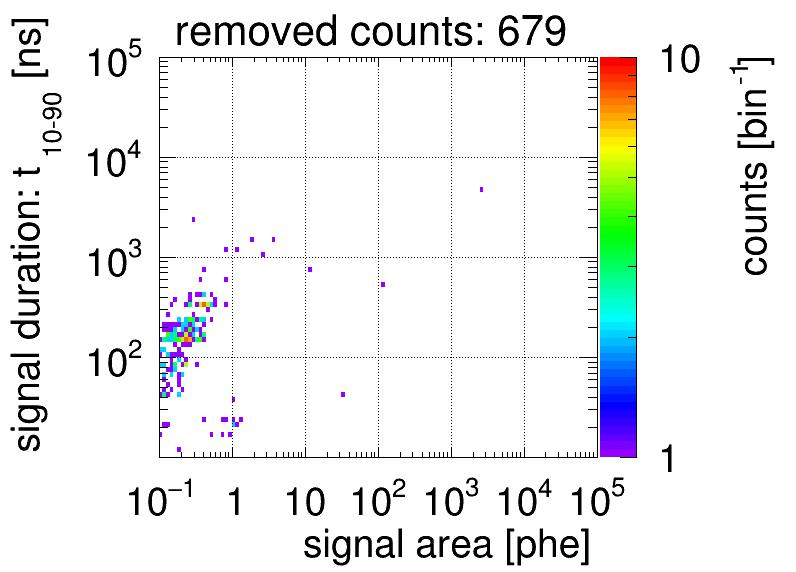
\includegraphics[width=\figurewidth,clip,trim={0 98 0 15}]{Figures/GasTest/CutsValid/res64767/pdpaX04Vecfig64767.jpg}
		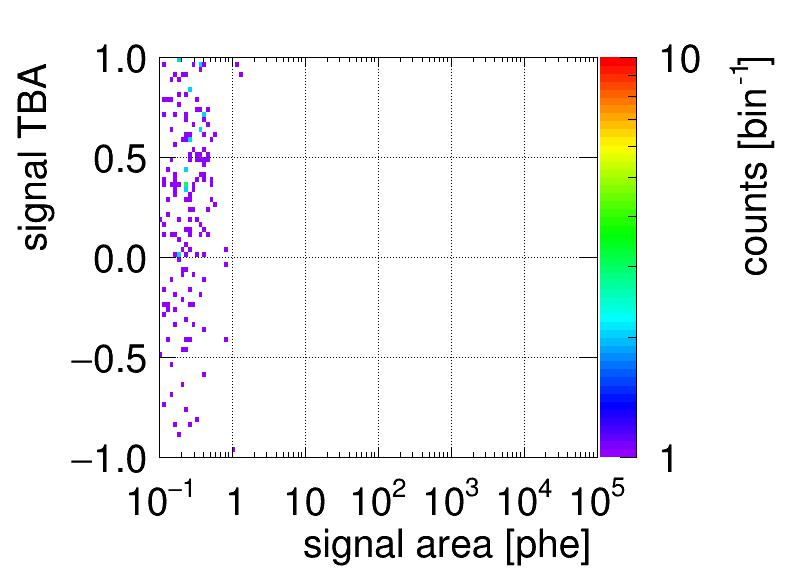
\includegraphics[width=\figurewidth,clip,trim={0 8 0 40}]{Figures/GasTest/CutsValid/res64767/tbapaX04Vecfig64767.jpg}
%		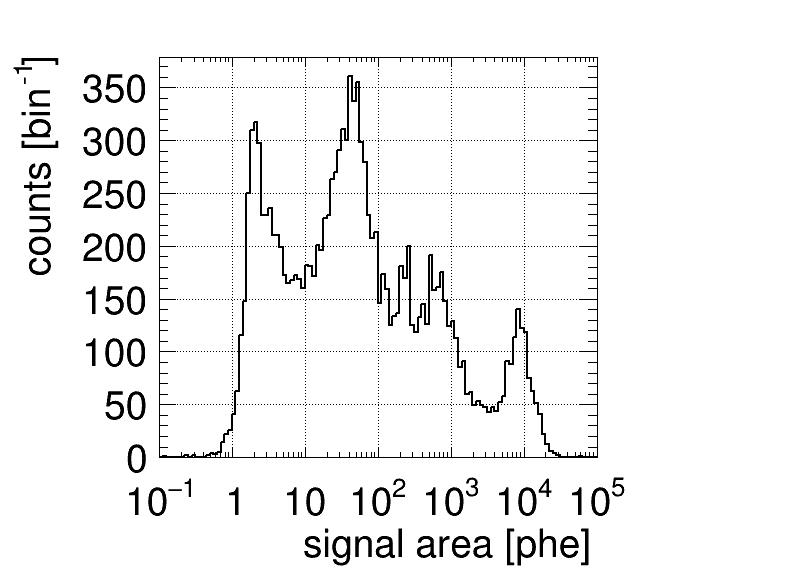
\includegraphics[width=\figurewidth,clip,trim={0 0 0 0}]{Figures/GasTest/CutsValid/res64767/pa04Vecfig64767.jpg}
		\caption{}
		\label{fig:signal selection 04}
	\end{subfigure}
	\begin{subfigure}[t]{0.32\textwidth}
	\centering
		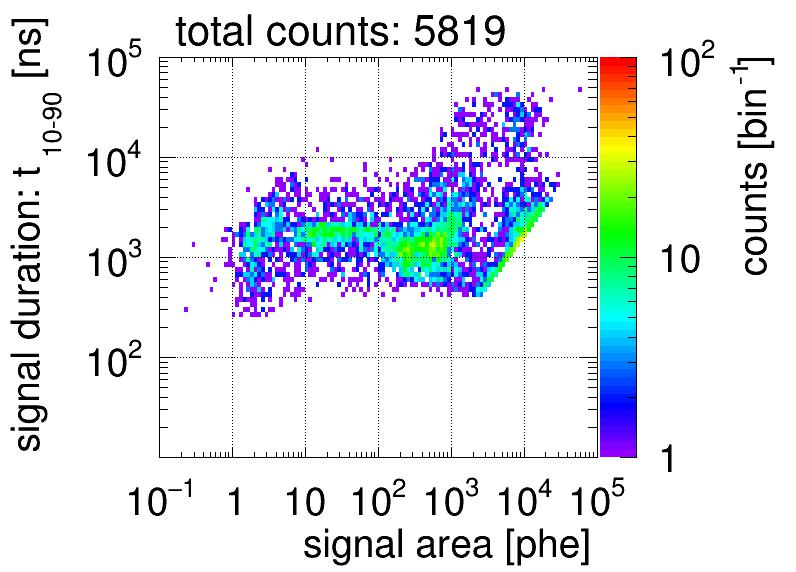
\includegraphics[width=\figurewidth,clip,trim={0 98 0 15}]{Figures/GasTest/CutsValid/res64767/pdpa05Vecfig64767.jpg}
		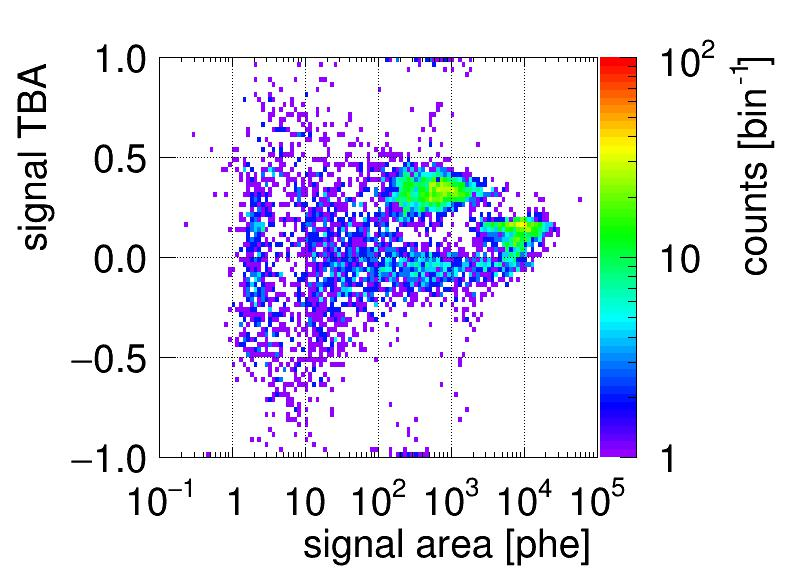
\includegraphics[width=\figurewidth,clip,trim={0 98 0 40}]{Figures/GasTest/CutsValid/res64767/tbapa05Vecfig64767.jpg}
		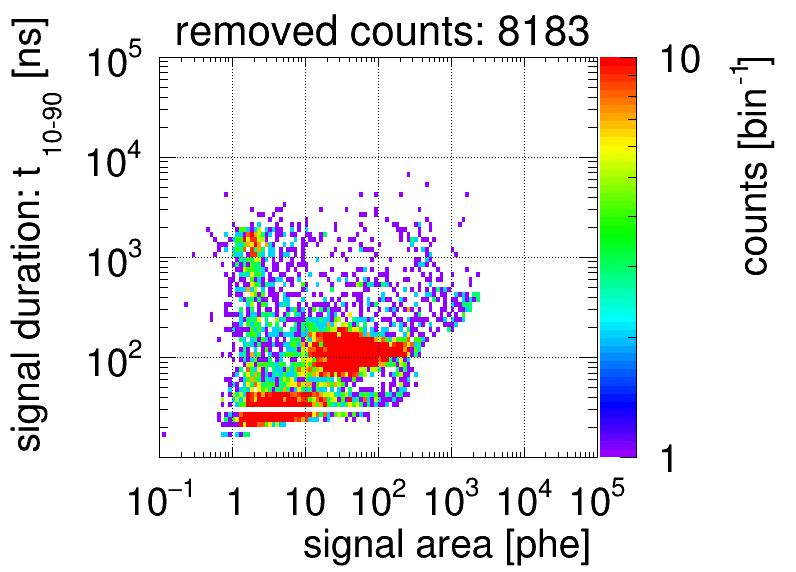
\includegraphics[width=\figurewidth,clip,trim={0 98 0 15}]{Figures/GasTest/CutsValid/res64767/pdpaX05Vecfig64767.jpg}
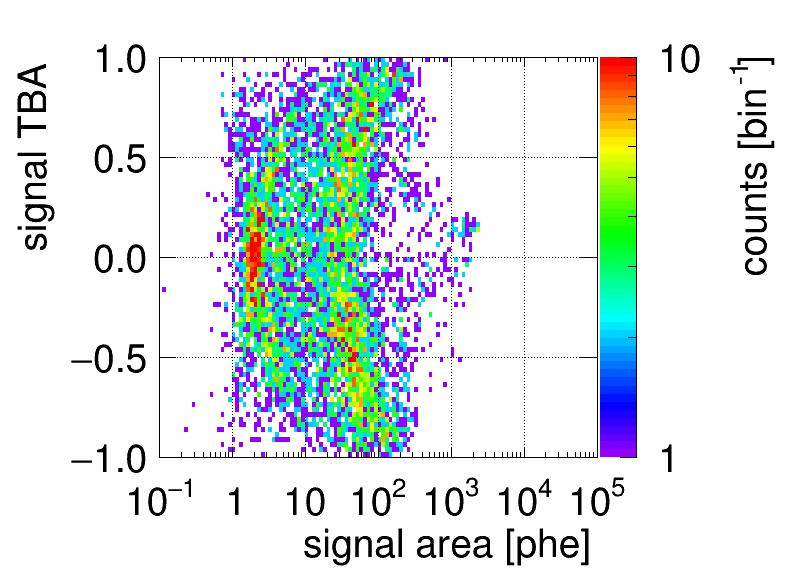
\includegraphics[width=\figurewidth,clip,trim={0 8 0 40}]{Figures/GasTest/CutsValid/res64767/tbapaX05Vecfig64767.jpg}
%		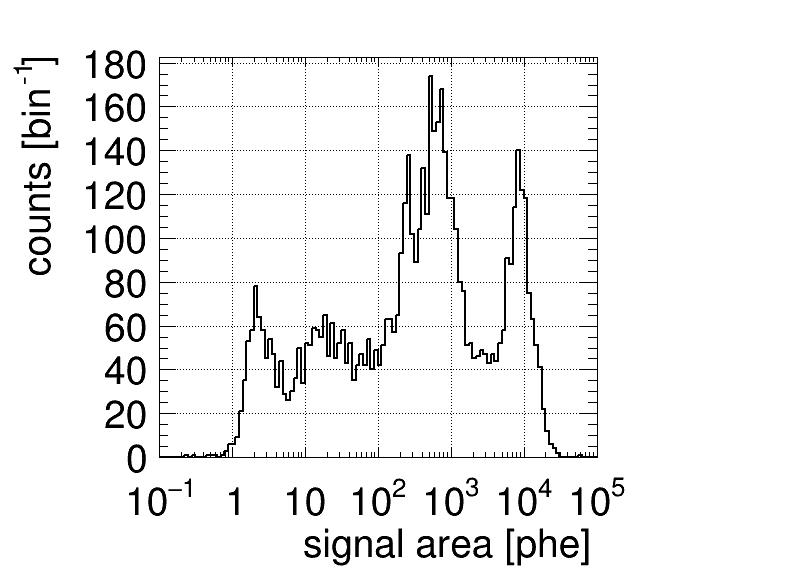
\includegraphics[width=\figurewidth,clip,trim={0 0 0 0}]{Figures/GasTest/CutsValid/res64767/pa05Vecfig64767.jpg}
	\caption{}
	\label{fig:signal selection 05}
\end{subfigure}
	\begin{subfigure}[t]{0.32\textwidth}
	\centering
	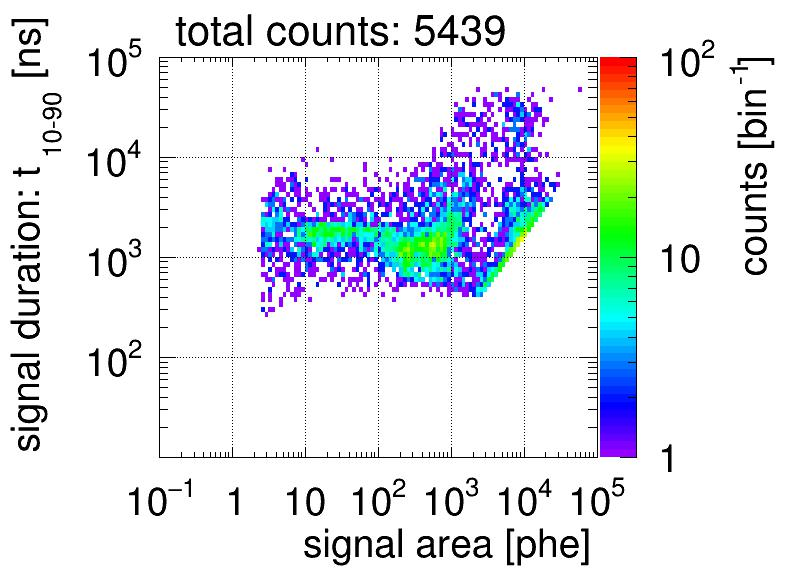
\includegraphics[width=\figurewidth,clip,trim={0 98 0 15}]{Figures/GasTest/CutsValid/res64767/pdpa06Vecfig64767.jpg}
	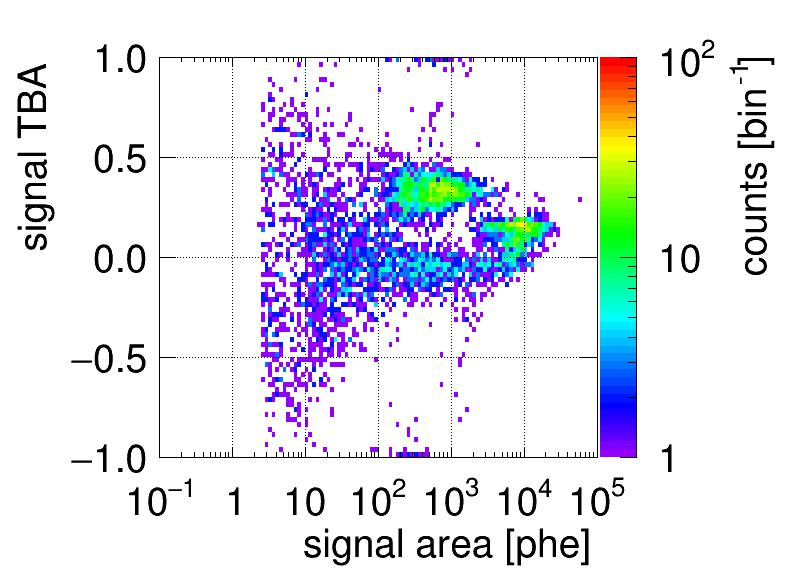
\includegraphics[width=\figurewidth,clip,trim={0 98 0 40}]{Figures/GasTest/CutsValid/res64767/tbapa06Vecfig64767.jpg}
	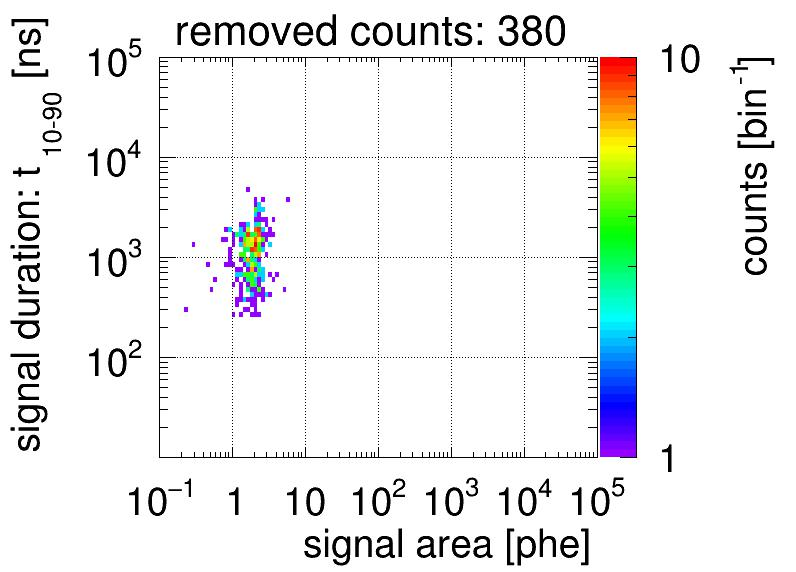
\includegraphics[width=\figurewidth,clip,trim={0 98 0 15}]{Figures/GasTest/CutsValid/res64767/pdpaX06Vecfig64767.jpg}
	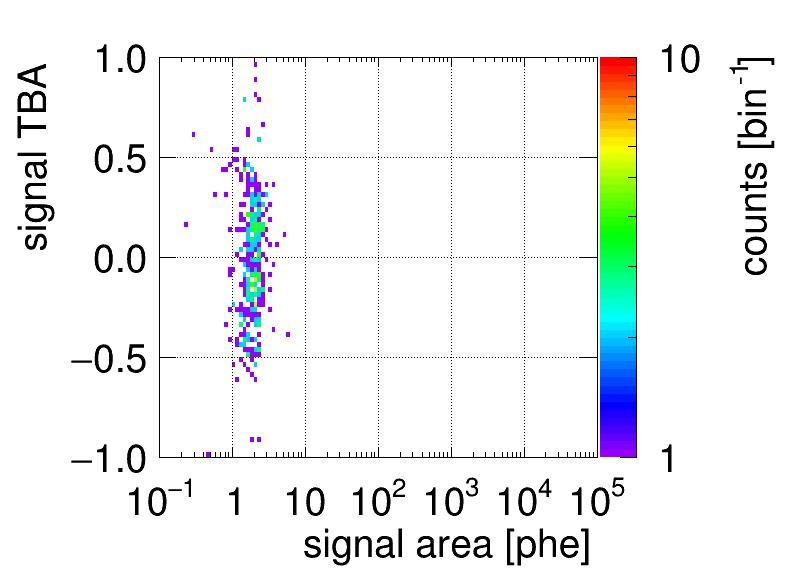
\includegraphics[width=\figurewidth,clip,trim={0 8 0 40}]{Figures/GasTest/CutsValid/res64767/tbapaX06Vecfig64767.jpg}
	%		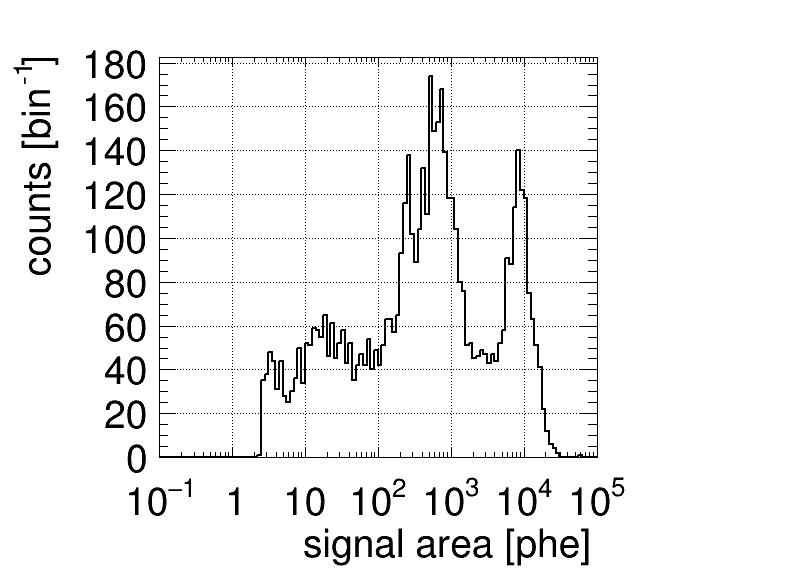
\includegraphics[width=\figurewidth,clip,trim={0 0 0 0}]{Figures/GasTest/CutsValid/res64767/pa06Vecfig64767.jpg}
	\caption{}
	\label{fig:signal selection 06}
\end{subfigure}
	\caption[\gtest\ signal selection (part~1).]{\gtest\ signal selection (part~1): 
			(row one) distribution of \rpdshort\ vs area after signal selections;
(row two) distribution of TBA vs area after signal selections;
(row three) distribution of \rpdshort\ vs area of removed signals;
(row four) distribution of TBA vs area of removed signals;
		(a) coinciding event building; 
		(b) applying signal selections up to ``not a noise-like signal";
		(c) applying signal selections up to ``not a narrow (S1-like) signal";
		(d) applying signal selections up to ``not a two-\sphe\ accidental coinciding signal".
		The cuts described in the text are applied successively from panel to panel. See the main text for detailed descriptions of the event populations.
		Data were taken at \ddtt{2017}{12}{08}{14}{02}, with \opvtvb\ at \SIlist{+6;-6}{kV}, \opgd\ at \standarddensity . The duration of data taking is \SI{180.09}{\s}.
     }
	\label{fig:signal selection l1}
\end{figure}
\end{landscape}
\begin{landscape}
	\begin{figure}[!p]\ContinuedFloat
		\centering
		\begin{subfigure}[t]{0.32\textwidth} %0.44\textwidth is the maximum to fit three column in a row
			\centering
			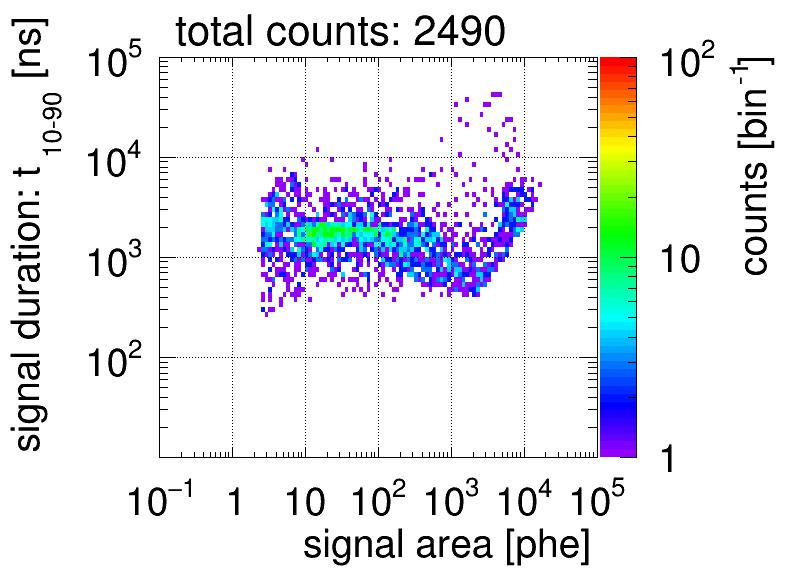
\includegraphics[width=\figurewidth,clip,trim={0 98 0 15}]{Figures/GasTest/CutsValid/res64767/pdpa07Vecfig64767.jpg}
			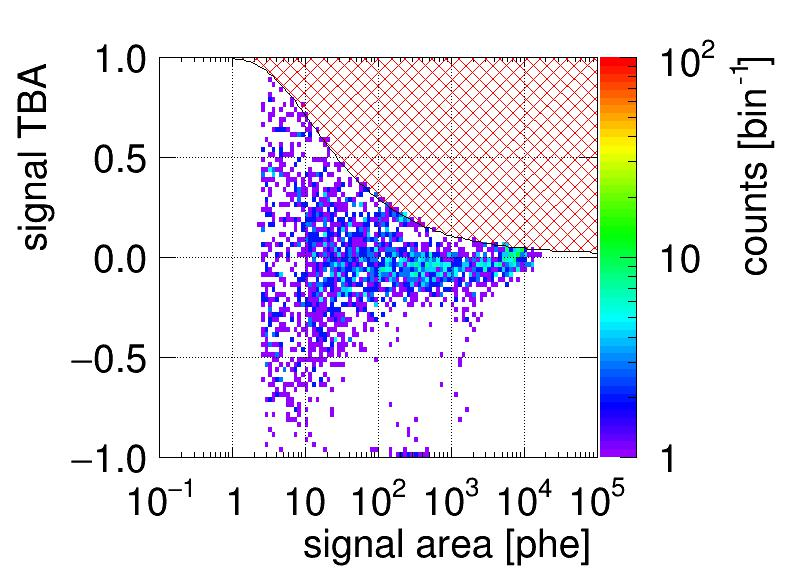
\includegraphics[width=\figurewidth,clip,trim={0 98 0 40}]{Figures/GasTest/CutsValid/res64767/tbapa07Vecfig64767.jpg}
			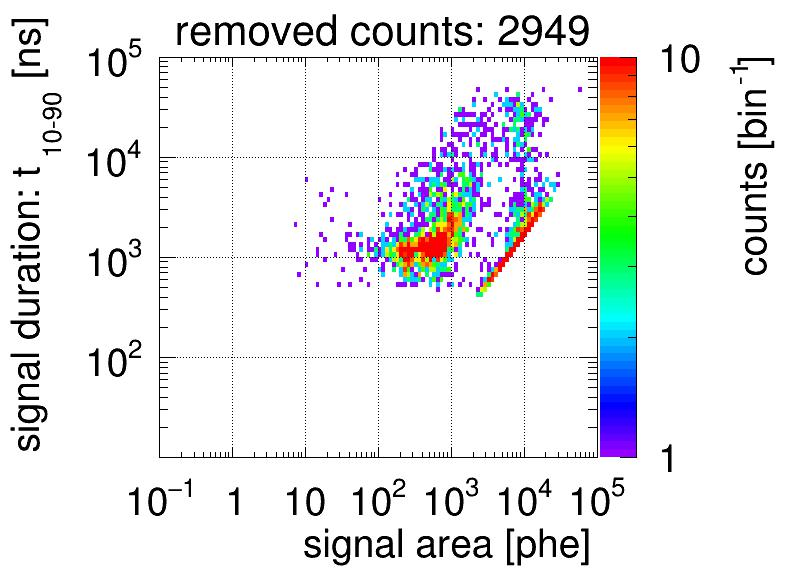
\includegraphics[width=\figurewidth,clip,trim={0 98 0 15}]{Figures/GasTest/CutsValid/res64767/pdpaX07Vecfig64767.jpg}
			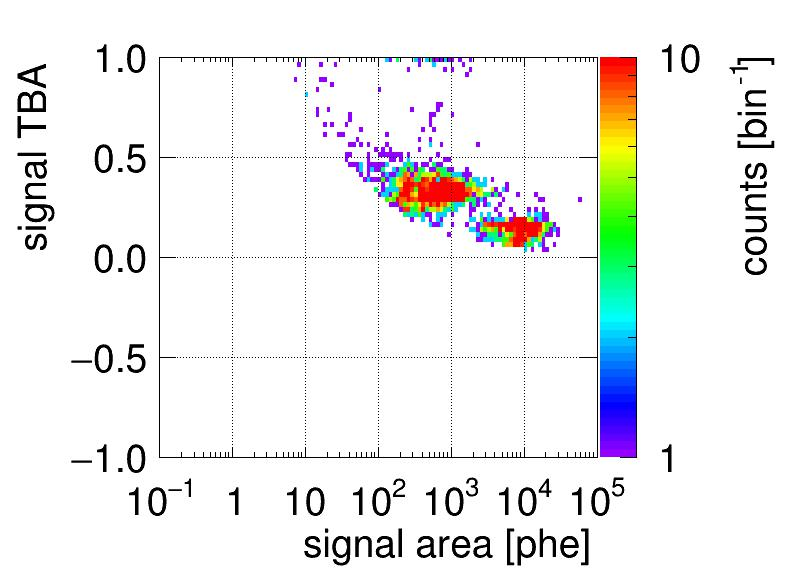
\includegraphics[width=\figurewidth,clip,trim={0 8 0 40}]{Figures/GasTest/CutsValid/res64767/tbapaX07Vecfig64767.jpg}
			%		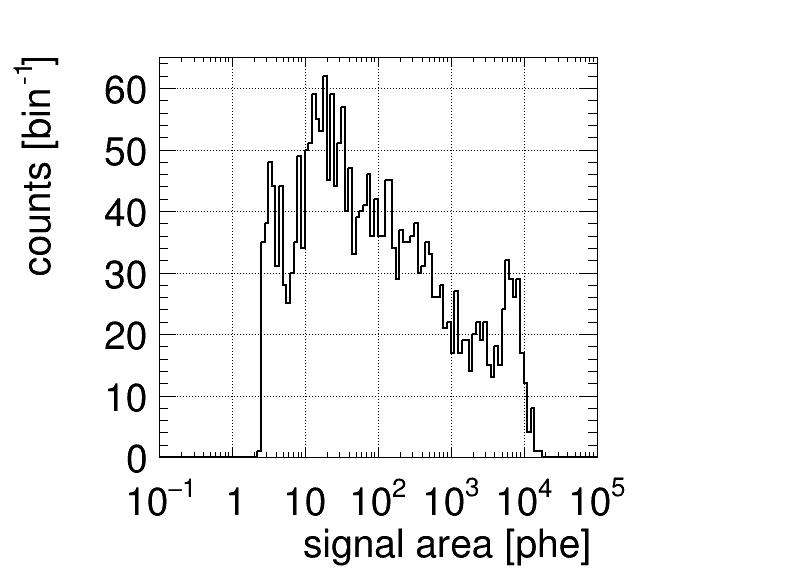
\includegraphics[width=\figurewidth,clip,trim={0 0 0 0}]{Figures/GasTest/CutsValid/res64767/pa07Vecfig64767.jpg}
			\caption{}
			\label{fig:signal selection 07}
		\end{subfigure}
		\begin{subfigure}[t]{0.32\textwidth}
			\centering
			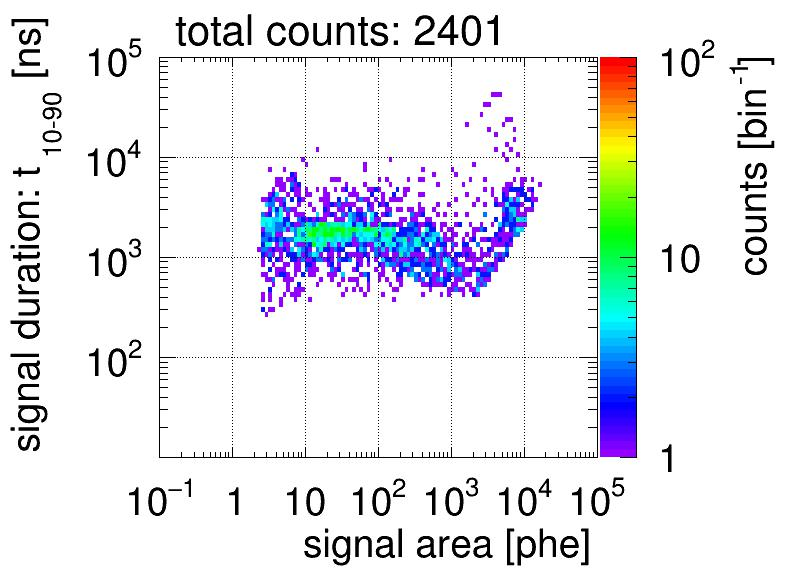
\includegraphics[width=\figurewidth,clip,trim={0 98 0 15}]{Figures/GasTest/CutsValid/res64767/pdpa08Vecfig64767.jpg}
			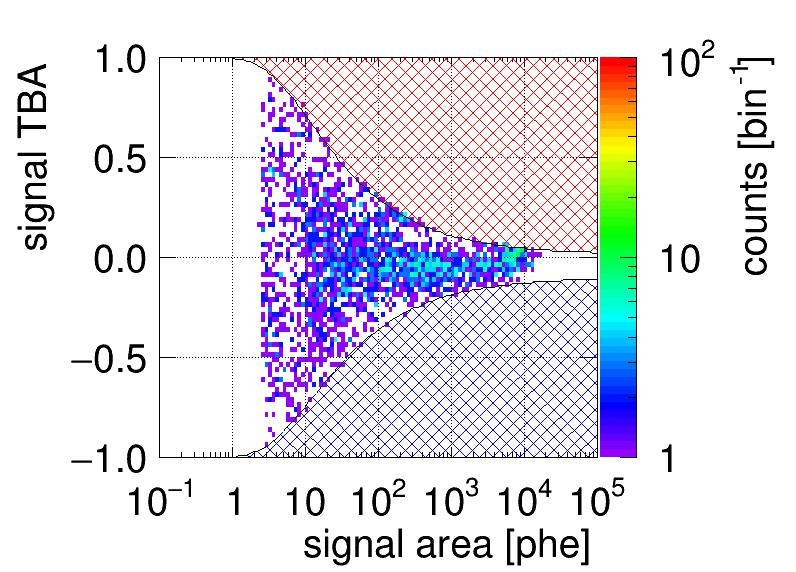
\includegraphics[width=\figurewidth,clip,trim={0 98 0 40}]{Figures/GasTest/CutsValid/res64767/tbapa08Vecfig64767.jpg}
			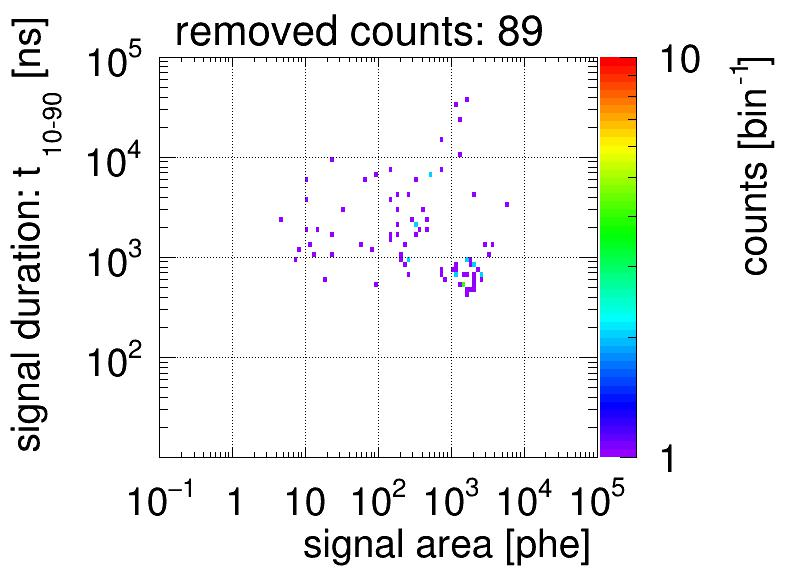
\includegraphics[width=\figurewidth,clip,trim={0 98 0 15}]{Figures/GasTest/CutsValid/res64767/pdpaX08Vecfig64767.jpg}
			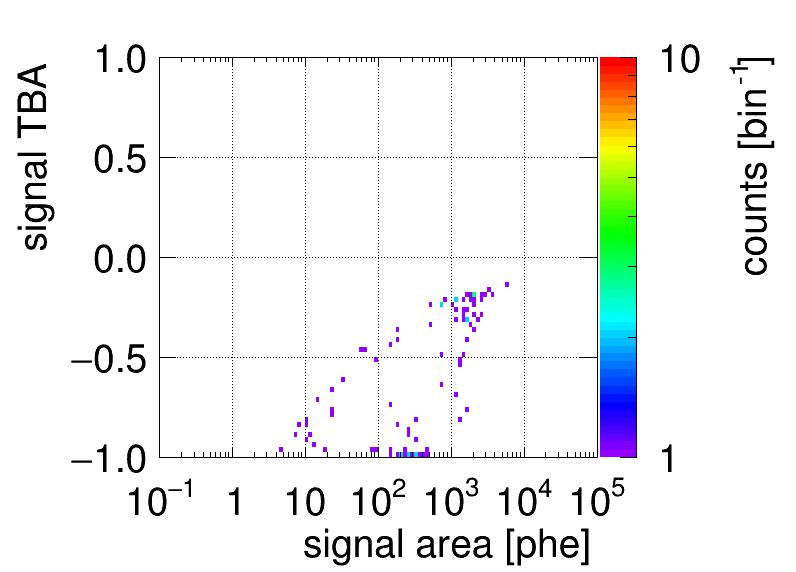
\includegraphics[width=\figurewidth,clip,trim={0 8 0 40}]{Figures/GasTest/CutsValid/res64767/tbapaX08Vecfig64767.jpg}
			%		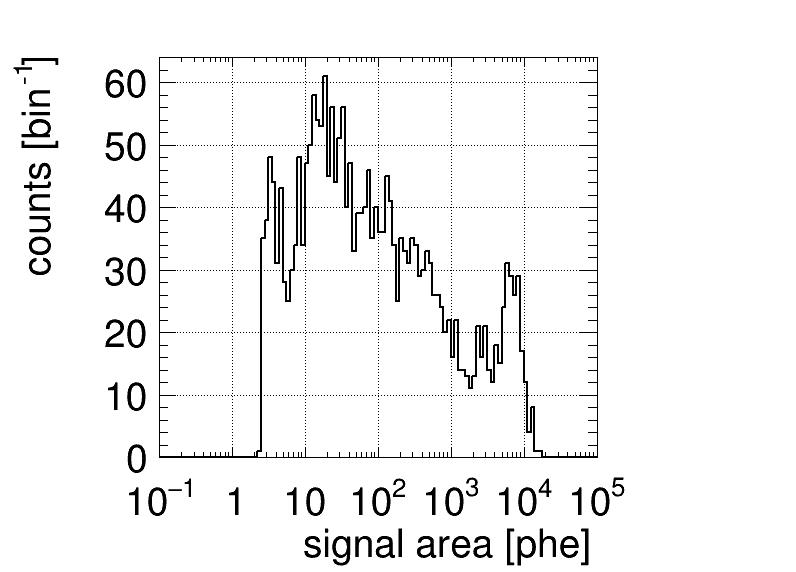
\includegraphics[width=\figurewidth,clip,trim={0 0 0 0}]{Figures/GasTest/CutsValid/res64767/pa08Vecfig64767.jpg}
			\caption{}
			\label{fig:signal selection 08}
		\end{subfigure}
		\begin{subfigure}[t]{0.32\textwidth}
			\centering
			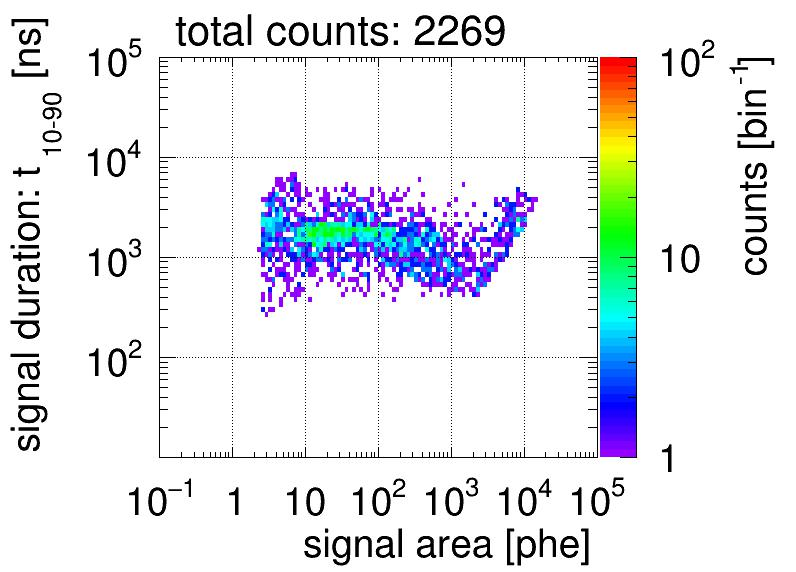
\includegraphics[width=\figurewidth,clip,trim={0 98 0 15}]{Figures/GasTest/CutsValid/res64767/pdpa09Vecfig64767.jpg}
			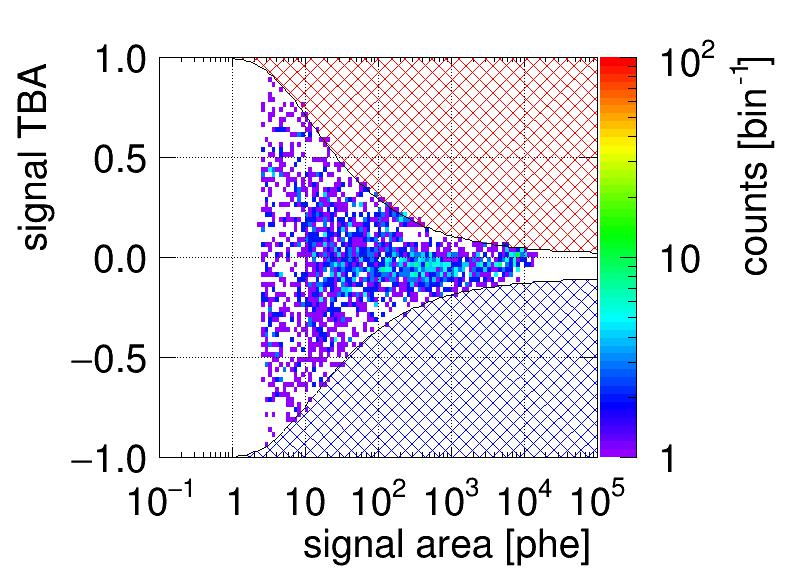
\includegraphics[width=\figurewidth,clip,trim={0 98 0 40}]{Figures/GasTest/CutsValid/res64767/tbapa09Vecfig64767.jpg}
			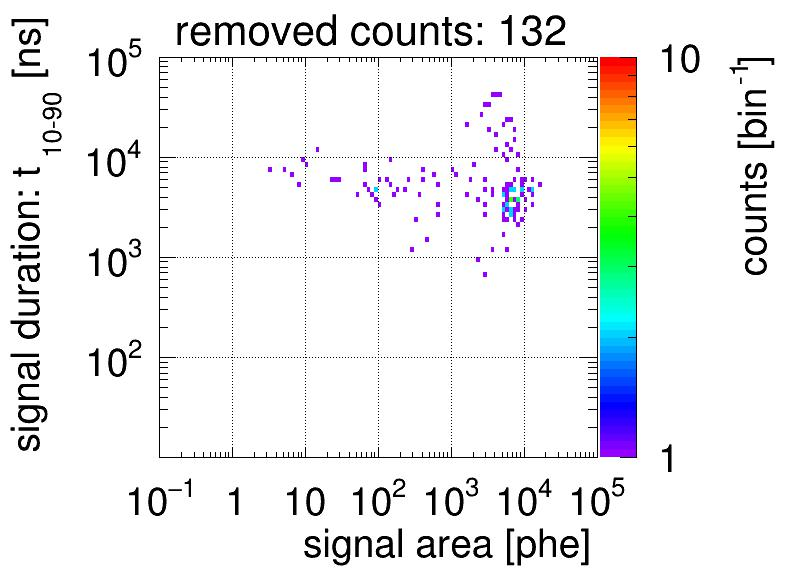
\includegraphics[width=\figurewidth,clip,trim={0 98 0 15}]{Figures/GasTest/CutsValid/res64767/pdpaX09Vecfig64767.jpg}
			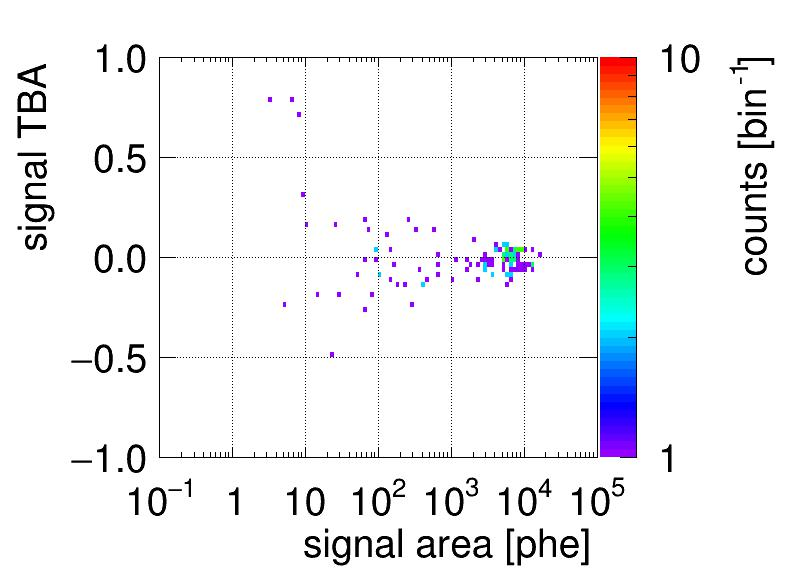
\includegraphics[width=\figurewidth,clip,trim={0 8 0 40}]{Figures/GasTest/CutsValid/res64767/tbapaX09Vecfig64767.jpg}
			%		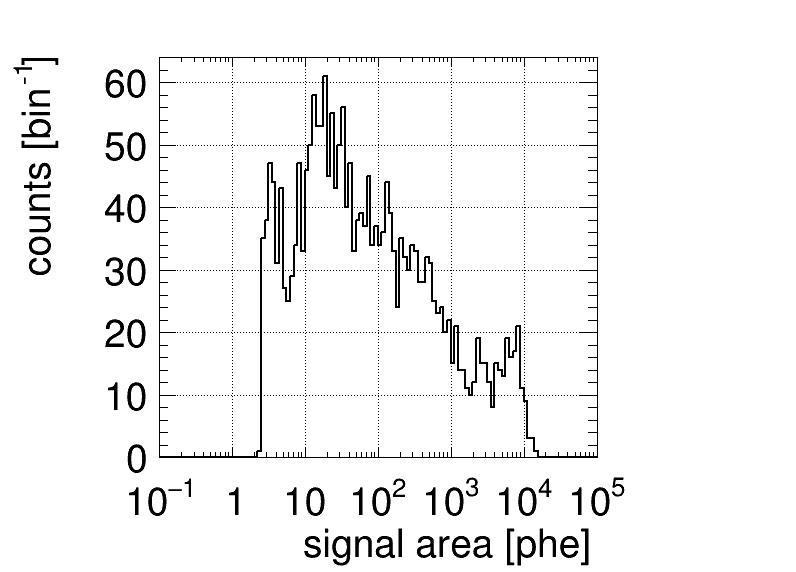
\includegraphics[width=\figurewidth,clip,trim={0 0 0 0}]{Figures/GasTest/CutsValid/res64767/pa09Vecfig64767.jpg}
			\caption{}
			\label{fig:signal selection 09}
		\end{subfigure}
		\begin{subfigure}[t]{0.32\textwidth}
			\centering
			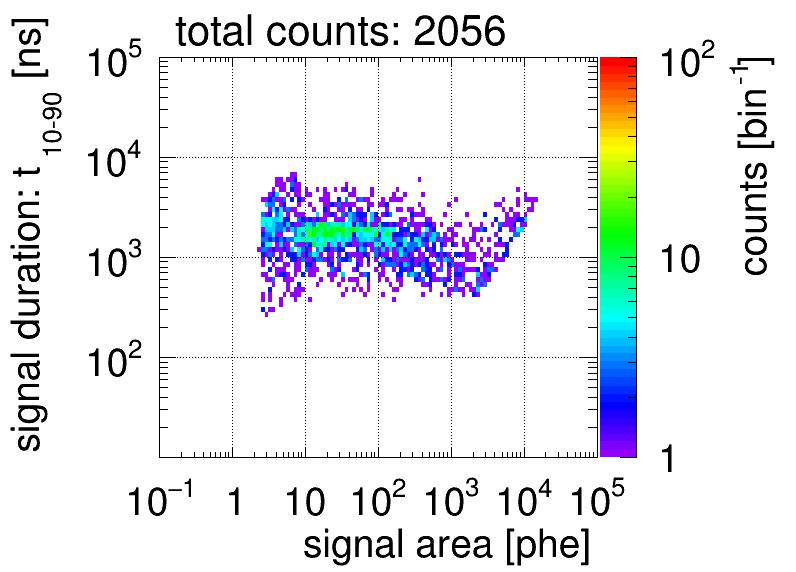
\includegraphics[width=\figurewidth,clip,trim={0 98 0 15}]{Figures/GasTest/CutsValid/res64767/pdpa10Vecfig64767.jpg}
			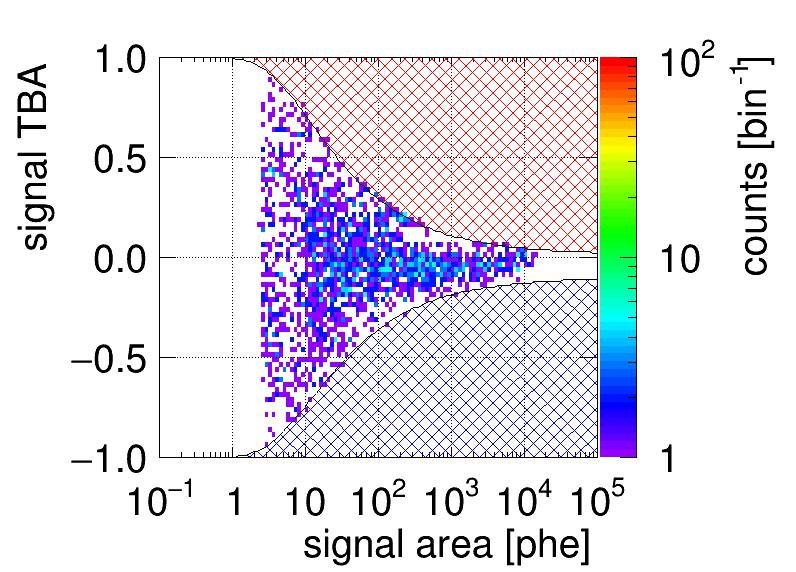
\includegraphics[width=\figurewidth,clip,trim={0 98 0 40}]{Figures/GasTest/CutsValid/res64767/tbapa10Vecfig64767.jpg}
			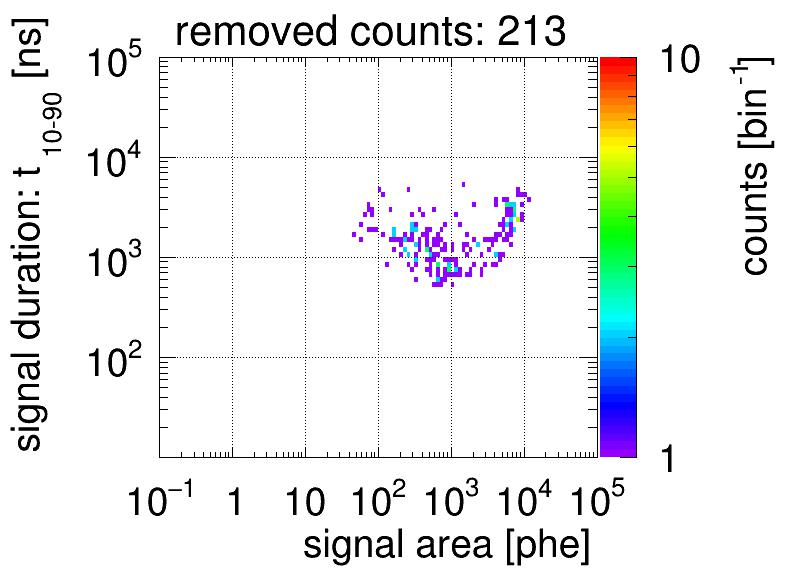
\includegraphics[width=\figurewidth,clip,trim={0 98 0 15}]{Figures/GasTest/CutsValid/res64767/pdpaX10Vecfig64767.jpg}
			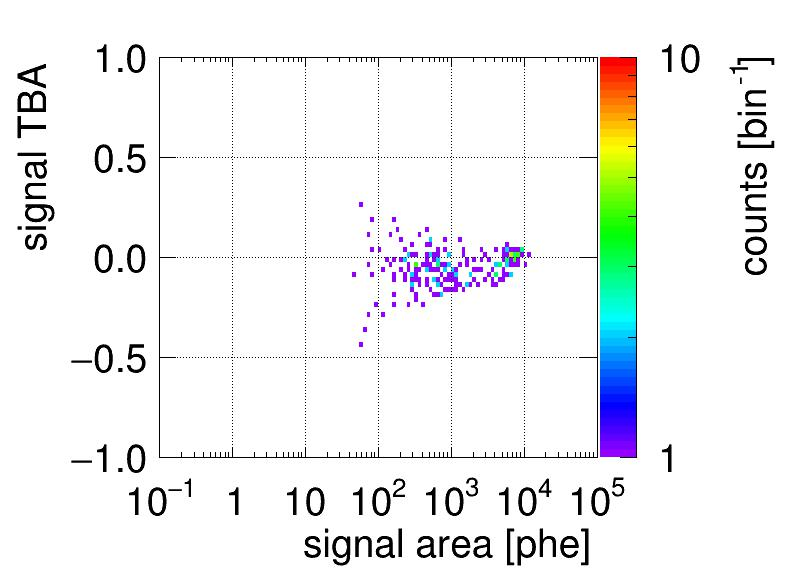
\includegraphics[width=\figurewidth,clip,trim={0 8 0 40}]{Figures/GasTest/CutsValid/res64767/tbapaX10Vecfig64767.jpg}
			%		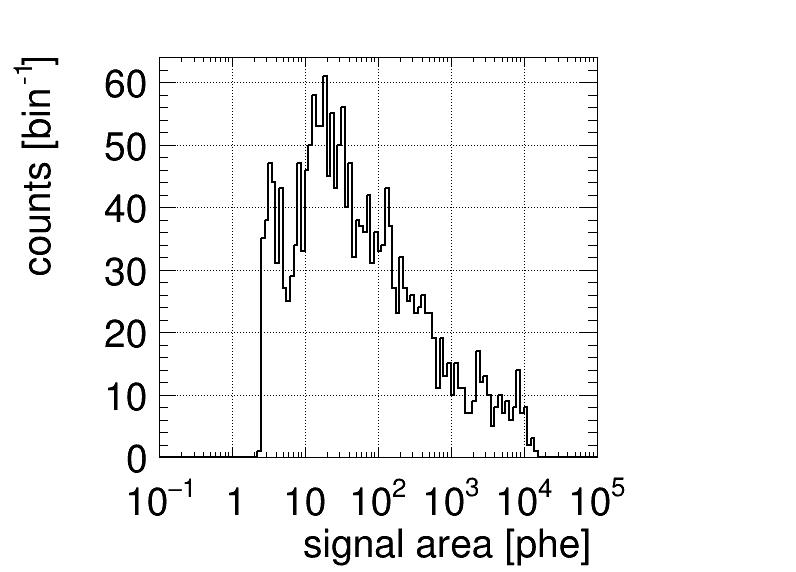
\includegraphics[width=\figurewidth,clip,trim={0 0 0 0}]{Figures/GasTest/CutsValid/res64767/pa10Vecfig64767.jpg}
			\caption{}
			\label{fig:signal selection 10}
		\end{subfigure}
		\caption[\gtest\ signal selection (part~2).]{\gtest\ signal selection (part~2): 
			(row one) distribution of \rpdshort\ vs area after signal selections;
(row two) distribution of TBA vs area after signal selections;
(row three) distribution of \rpdshort\ vs area of removed signals;
(row four) distribution of TBA vs area of removed signals;
(e) applying signal selections up to ``not a top-heavy signal";
(f) applying signal selections up to ``not a bottom-heavy signal";
(g) applying signal selections up to ``not a extremely long duration signal";
(h) applying signal selections up to ``not a right-angled triangle shape signal".
The red hatched shaded area indicates the ``top-heavy" region.
The blue shaded area indicates the ``bottom-heavy" region.
		The cuts described in the text are applied successively from panel to panel. See the main text for detailed descriptions of the event populations.
		Data were taken at \ddtt{2017}{12}{08}{14}{02}, with \opvtvb\ at \SIlist{+6;-6}{kV}, \opgd\ at \standarddensity . The duration of data taking is \SI{180.09}{\s}.
		}
		\label{fig:signal selection l2}
	\end{figure}
\end{landscape}
\begin{landscape}
	\begin{figure}[!p]\ContinuedFloat
	\centering
	\begin{subfigure}[t]{0.32\textwidth} %0.44\textwidth is the maximum to fit three column in a row
		\centering
		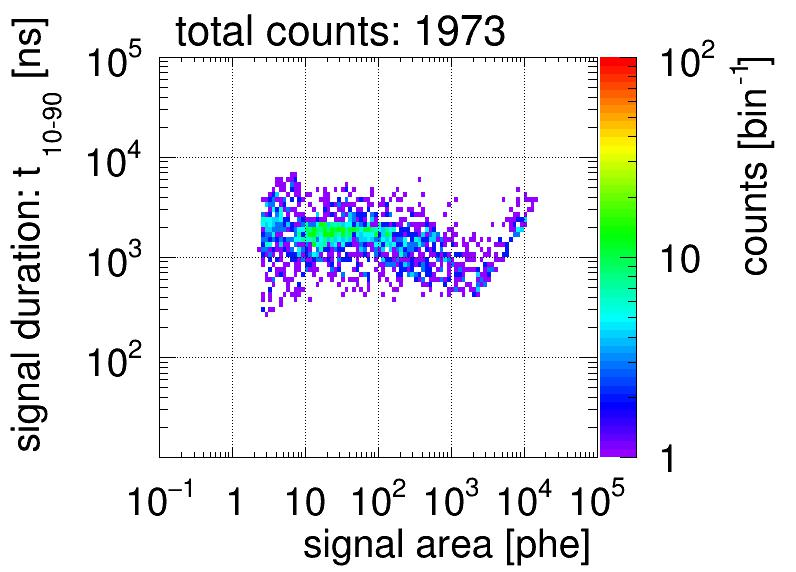
\includegraphics[width=\figurewidth,clip,trim={0 98 0 15}]{Figures/GasTest/CutsValid/res64767/pdpa11Vecfig64767.jpg}
		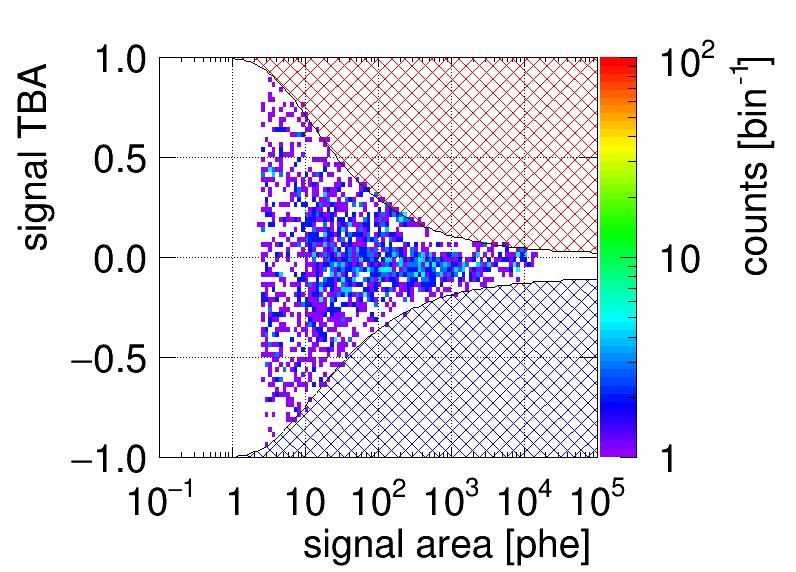
\includegraphics[width=\figurewidth,clip,trim={0 98 0 40}]{Figures/GasTest/CutsValid/res64767/tbapa11Vecfig64767.jpg}
		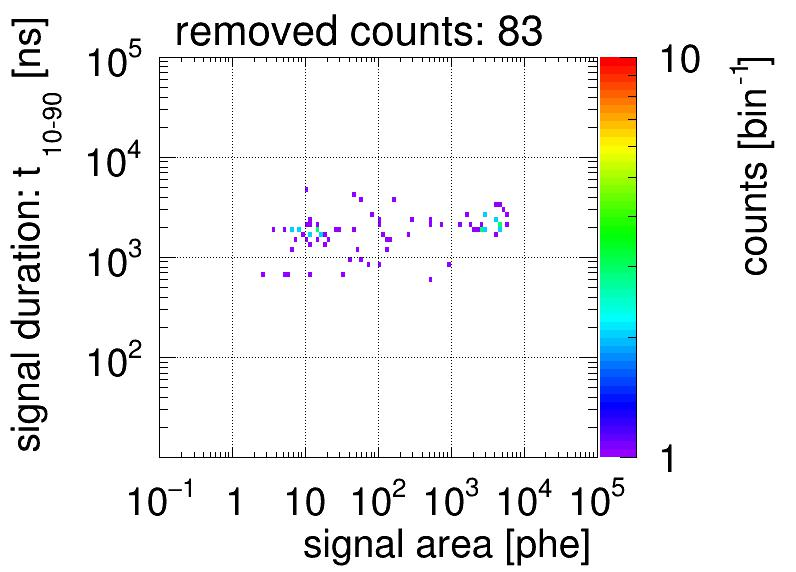
\includegraphics[width=\figurewidth,clip,trim={0 98 0 15}]{Figures/GasTest/CutsValid/res64767/pdpaX11Vecfig64767.jpg}
		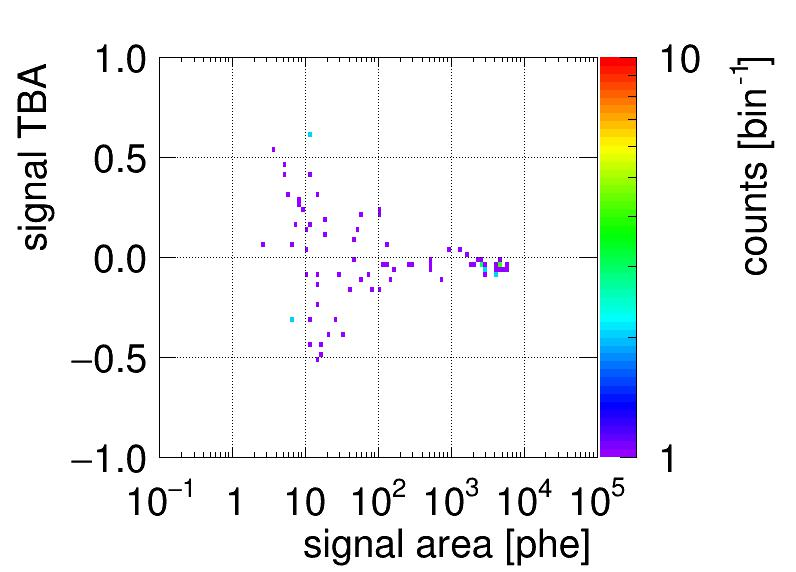
\includegraphics[width=\figurewidth,clip,trim={0 8 0 40}]{Figures/GasTest/CutsValid/res64767/tbapaX11Vecfig64767.jpg}
		%		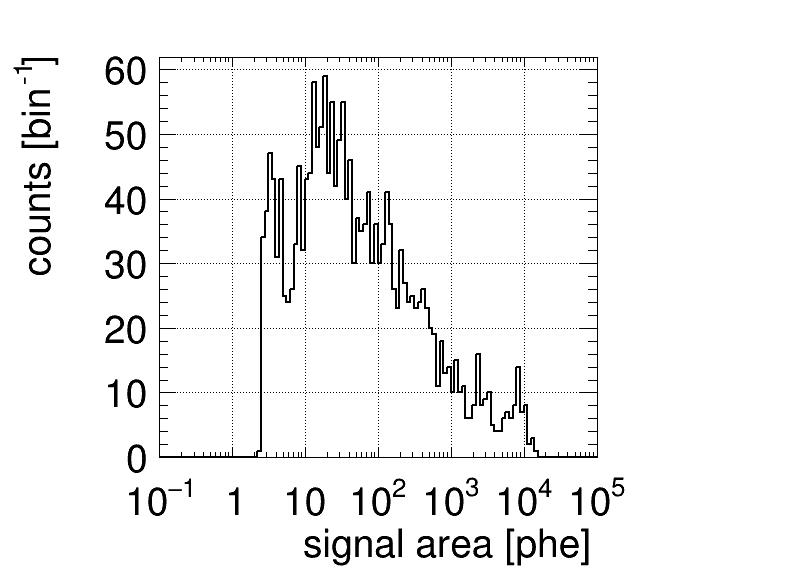
\includegraphics[width=\figurewidth,clip,trim={0 0 0 0}]{Figures/GasTest/CutsValid/res64767/pa11Vecfig64767.jpg}
		\caption{}
		\label{fig:signal selection 11}
	\end{subfigure}
	\begin{subfigure}[t]{0.32\textwidth}
		\centering
		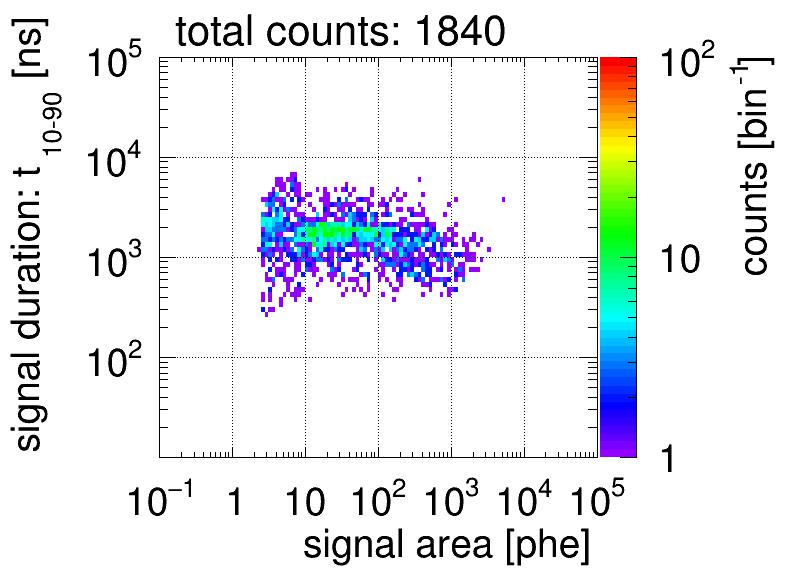
\includegraphics[width=\figurewidth,clip,trim={0 98 0 15}]{Figures/GasTest/CutsValid/res64767/pdpa12Vecfig64767.jpg}
		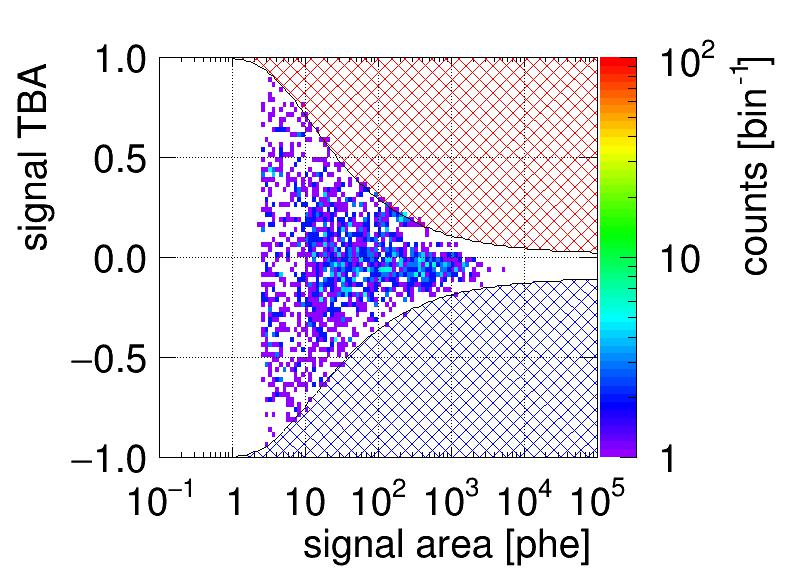
\includegraphics[width=\figurewidth,clip,trim={0 98 0 40}]{Figures/GasTest/CutsValid/res64767/tbapa12Vecfig64767.jpg}
		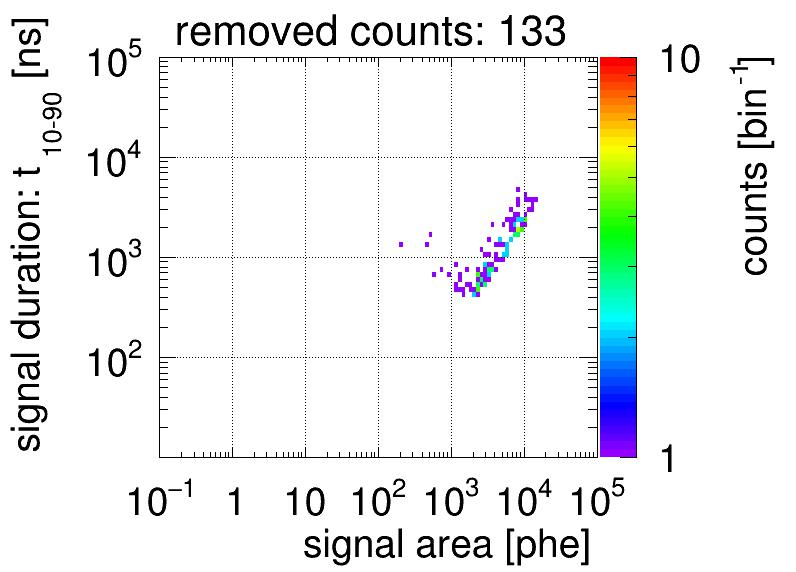
\includegraphics[width=\figurewidth,clip,trim={0 98 0 15}]{Figures/GasTest/CutsValid/res64767/pdpaX12Vecfig64767.jpg}
		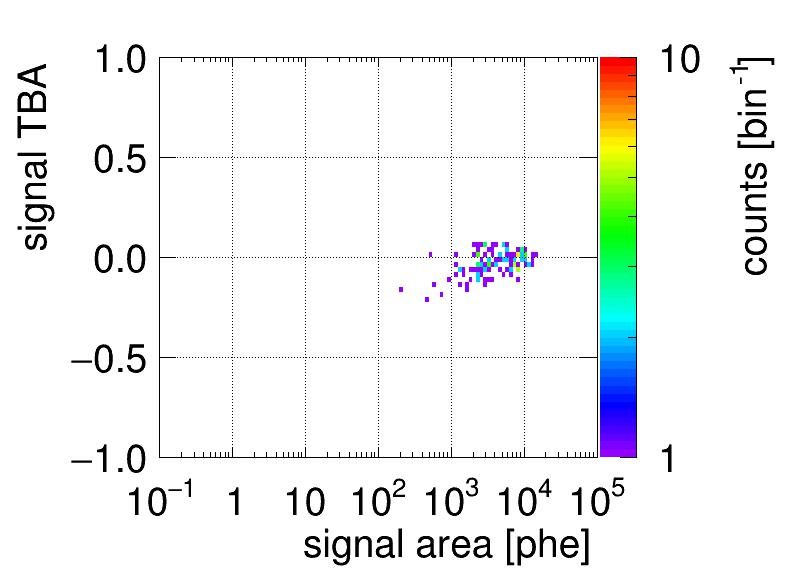
\includegraphics[width=\figurewidth,clip,trim={0 8 0 40}]{Figures/GasTest/CutsValid/res64767/tbapaX12Vecfig64767.jpg}
		%		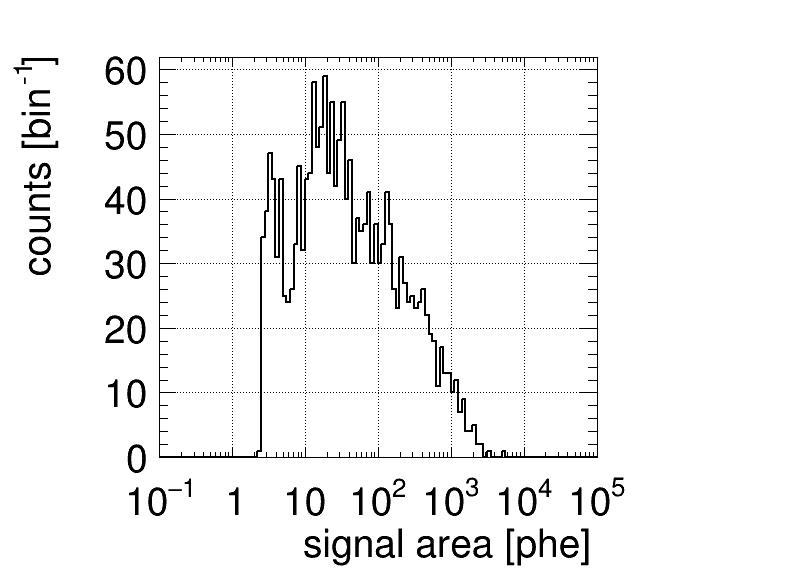
\includegraphics[width=\figurewidth,clip,trim={0 0 0 0}]{Figures/GasTest/CutsValid/res64767/pa12Vecfig64767.jpg}
		\caption{}
		\label{fig:signal selection 12}
	\end{subfigure}
	\begin{subfigure}[t]{0.32\textwidth}
		\centering
		\includegraphics[width=\figurewidth,clip,trim={0 98 0 15}]{Figures/GasTest/CutsValid/res64767/pdpa13Vecfig64767.jpg}
		\includegraphics[width=\figurewidth,clip,trim={0 98 0 40}]{Figures/GasTest/CutsValid/res64767/tbapa13Vecfig64767.jpg}
		\includegraphics[width=\figurewidth,clip,trim={0 98 0 15}]{Figures/GasTest/CutsValid/res64767/pdpaX13Vecfig64767.jpg}
		\includegraphics[width=\figurewidth,clip,trim={0 8 0 40}]{Figures/GasTest/CutsValid/res64767/tbapaX13Vecfig64767.jpg}
		%		\includegraphics[width=\figurewidth,clip,trim={0 0 0 0}]{Figures/GasTest/CutsValid/res64767/pa13Vecfig64767.jpg}
		\caption{}
		\label{fig:signal selection 13}
	\end{subfigure}
	\begin{subfigure}[t]{0.32\textwidth}
		\centering
		\includegraphics[width=\figurewidth,clip,trim={0 98 0 15}]{Figures/GasTest/CutsValid/res64767/pdpa14Vecfig64767.jpg}
		\includegraphics[width=\figurewidth,clip,trim={0 98 0 40}]{Figures/GasTest/CutsValid/res64767/tbapa14Vecfig64767.jpg}
		\includegraphics[width=\figurewidth,clip,trim={0 98 0 15}]{Figures/GasTest/CutsValid/res64767/pdpaX14Vecfig64767.jpg}
		\includegraphics[width=\figurewidth,clip,trim={0 8 0 40}]{Figures/GasTest/CutsValid/res64767/tbapaX14Vecfig64767.jpg}
		%		\includegraphics[width=\figurewidth,clip,trim={0 0 0 0}]{Figures/GasTest/CutsValid/res64767/pa14Vecfig64767.jpg}
		\caption{}
		\label{fig:signal selection 14}
	\end{subfigure}
	\caption[\gtest\ signal selection (part~3).]{\gtest\ signal selection (part~3): 
			(row one) distribution of \rpdshort\ vs area after signal selections;
(row two) distribution of TBA vs area after signal selections;
(row three) distribution of \rpdshort\ vs area of removed signals;
(row four) distribution of TBA vs area of removed signals;
(i) applying signal selections up to ``not an S1 S2 like signal";
(j) applying signal selections up to ``not a saturated signal";
(k) applying signal selections up to ``not a long duration signal";
(l) applying signal selections up to ``not a short duration signal".
The red hatched shaded area indicates the ``top-heavy" region.
The blue shaded area indicates the ``bottom-heavy" region.
The magenta hatched shaded area indicates the ``long duration" region.
The cyan hatched shaded area indicates the ``short duration" region.
		The cuts described in the text are applied successively from panel to panel. See the main text for detailed descriptions of the event populations.
		Data were taken at \ddtt{2017}{12}{08}{14}{02}, with \opvtvb\ at \SIlist{+6;-6}{kV}, \opgd\ at \standarddensity . The duration of data taking is \SI{180.09}{\s}.
	}
	\label{fig:signal selection l3}
\end{figure}
\end{landscape}
\begin{landscape}
	\begin{figure}[!p]\ContinuedFloat
	\centering
	\begin{subfigure}[t]{0.32\textwidth}
		\centering
		\includegraphics[width=\figurewidth,clip,trim={0 98 0 15}]{Figures/GasTest/CutsValid/res64767/pdpa15Vecfig64767.jpg}
		\includegraphics[width=\figurewidth,clip,trim={0 98 0 40}]{Figures/GasTest/CutsValid/res64767/tbapa15Vecfig64767.jpg}
		\includegraphics[width=\figurewidth,clip,trim={0 98 0 15}]{Figures/GasTest/CutsValid/res64767/pdpaX15Vecfig64767.jpg}
		\includegraphics[width=\figurewidth,clip,trim={0 8 0 40}]{Figures/GasTest/CutsValid/res64767/tbapaX15Vecfig64767.jpg}
		%		\includegraphics[width=\figurewidth,clip,trim={0 0 0 0}]{Figures/GasTest/CutsValid/res64767/pa15Vecfig64767.jpg}
		\caption{}
		\label{fig:signal selection 15}
	\end{subfigure}
	\begin{subfigure}[t]{0.32\textwidth}
	\centering
	\includegraphics[width=\figurewidth,clip,trim={0 98 0 15}]{Figures/GasTest/CutsValid/res64767/pdpa16Vecfig64767.jpg}
	\includegraphics[width=\figurewidth,clip,trim={0 98 0 40}]{Figures/GasTest/CutsValid/res64767/tbapa16Vecfig64767.jpg}
	\includegraphics[width=\figurewidth,clip,trim={0 98 0 15}]{Figures/GasTest/CutsValid/res64767/pdpaX16Vecfig64767.jpg}
	\includegraphics[width=\figurewidth,clip,trim={0 8 0 40}]{Figures/GasTest/CutsValid/res64767/tbapaX16Vecfig64767.jpg}
	%		\includegraphics[width=\figurewidth,clip,trim={0 0 0 0}]{Figures/GasTest/CutsValid/res64767/pa16Vecfig64767.jpg}
	\caption{}
	\label{fig:signal selection 16}
\end{subfigure}
	\caption[\gtest\ signal selection (part~4).]{\gtest\ signal selection (part~4): 
			(row one) distribution of \rpdshort\ vs area after signal selections;
			(row two) distribution of TBA vs area after signal selections;
			(row three) distribution of \rpdshort\ vs area of removed signals;
			(row four) distribution of TBA vs area of removed signals;
		(m) applying signal selections up to ``previous signal area veto".
				(n) applying signal selections up to ``Previous signal duration veto".
		The red hatched shaded area indicates the ``top-heavy" region.
		The blue shaded area indicates the ``bottom-heavy" region.
		The magenta hatched shaded area indicates the ``long duration" region.
		The cyan hatched shaded area indicates the ``short duration" region.
				The cuts described in the text are applied successively from panel to panel. See the main text for detailed descriptions of the event populations.
		Data were taken at \ddtt{2017}{12}{08}{14}{02}, with \opvtvb\ at \SIlist{+6;-6}{kV}, \opgd\ at \standarddensity . The duration of data taking is \SI{180.09}{\s}.
	}
	\label{fig:signal selection l4}
\end{figure}
\end{landscape}


\subsection{Signal selections varying \opdv\ and \opgd }
The results of signal selections 

\begin{landscape}%8kV
	\begin{figure}[!p]
		\centering
		\begin{subfigure}[t]{0.32\textwidth} %0.44\textwidth is the maximum to fit three column in a row
			\centering
			\includegraphics[width=\figurewidth,clip,trim={0 98 0 15}]{Figures/GasTest/CutsValid/res64765/pdpa22Vecfig64765.jpg}
			\includegraphics[width=\figurewidth,clip,trim={0 8 0 40}]{Figures/GasTest/CutsValid/res64765/tbapa22Vecfig64765.jpg}
			%		\includegraphics[width=\figurewidth,clip,trim={0 0 0 0}]{Figures/GasTest/CutsValid/res64765/pa22Vecfig64765.jpg}
			\caption{}
			\label{fig:signal selection dv 08 01}
		\end{subfigure}
		\begin{subfigure}[t]{0.32\textwidth}
			\centering
			\includegraphics[width=\figurewidth,clip,trim={0 98 0 15}]{Figures/GasTest/CutsValid/res64765/pdpa23Vecfig64765.jpg}
			\includegraphics[width=\figurewidth,clip,trim={0 98 0 40}]{Figures/GasTest/CutsValid/res64765/tbapa23Vecfig64765.jpg}
			\includegraphics[width=\figurewidth,clip,trim={0 98 0 15}]{Figures/GasTest/CutsValid/res64765/pdpaX23Vecfig64765.jpg}
			\includegraphics[width=\figurewidth,clip,trim={0 8 0 40}]{Figures/GasTest/CutsValid/res64765/tbapaX23Vecfig64765.jpg}
			%		\includegraphics[width=\figurewidth,clip,trim={0 0 0 0}]{Figures/GasTest/CutsValid/res64765/pa23Vecfig64765.jpg}
			\caption{}
			\label{fig:signal selection dv 08 02}
		\end{subfigure}
		\begin{subfigure}[t]{0.32\textwidth}
			\centering
			\includegraphics[width=\figurewidth,clip,trim={0 98 0 15}]{Figures/GasTest/CutsValid/res64765/pdpa26Vecfig64765.jpg}
			\includegraphics[width=\figurewidth,clip,trim={0 98 0 40}]{Figures/GasTest/CutsValid/res64765/tbapa26Vecfig64765.jpg}
			\includegraphics[width=\figurewidth,clip,trim={0 98 0 15}]{Figures/GasTest/CutsValid/res64765/pdpaX26Vecfig64765.jpg}
			\includegraphics[width=\figurewidth,clip,trim={0 8 0 40}]{Figures/GasTest/CutsValid/res64765/tbapaX26Vecfig64765.jpg}
			%		\includegraphics[width=\figurewidth,clip,trim={0 0 0 0}]{Figures/GasTest/CutsValid/res64765/pa26Vecfig64765.jpg}
			\caption{}
			\label{fig:signal selection dv 08 03}
		\end{subfigure}
		\begin{subfigure}[t]{0.32\textwidth}
			\centering
			\includegraphics[width=\figurewidth,clip,trim={0 98 0 15}]{Figures/GasTest/CutsValid/res64765/pdpa29Vecfig64765.jpg}
			\includegraphics[width=\figurewidth,clip,trim={0 98 0 40}]{Figures/GasTest/CutsValid/res64765/tbapa29Vecfig64765.jpg}
			\includegraphics[width=\figurewidth,clip,trim={0 98 0 15}]{Figures/GasTest/CutsValid/res64765/pdpaX29Vecfig64765.jpg}
			\includegraphics[width=\figurewidth,clip,trim={0 8 0 40}]{Figures/GasTest/CutsValid/res64765/tbapaX29Vecfig64765.jpg}
			%		\includegraphics[width=\figurewidth,clip,trim={0 0 0 0}]{Figures/GasTest/CutsValid/res64765/pa29Vecfig64765.jpg}
			\caption{}
			\label{fig:signal selection dv 08 04}
		\end{subfigure}
		\caption[\gtest\ signal selection with \opdv\ at \SI{8}{\kV}, \opgd\ at \standarddensity .]{\gtest\ signal selection with \opdv\ at \SI{8}{\kV}, \opgd\ at \standarddensity : 
			(row one) distribution of \rpdshort\ vs area after signal selections;
			(row two) distribution of TBA vs area after signal selections;
			(row three) distribution of \rpdshort\ vs area of removed signals;
			(row four) distribution of TBA vs area of removed signals;
			(a) coinciding event building; 
			(b) applying signal selections based on signal shape;
			(c) applying signal selections based on the previous signals;
			(d) applying signal selections based on signal shape and based on the previous signals.
			The red hatched shaded area indicates the ``top-heavy" region.
			The blue shaded area indicates the ``bottom-heavy" region.
			The magenta hatched shaded area indicates the ``long duration" region.
			The cyan hatched shaded area indicates the ``short duration" region.
			Data were taken at \ddtt{2017}{12}{08}{13}{43}, with \opvtvb\ at \SIlist{+4;-4}{kV}. The duration of data taking is \SI{179.95}{\s}.
		}
		\label{fig:signal selection dv 08}
	\end{figure}
\end{landscape}
\begin{landscape}%10kV
	\begin{figure}[!p]
		\centering
		\begin{subfigure}[t]{0.32\textwidth} %0.44\textwidth is the maximum to fit three column in a row
			\centering
			\includegraphics[width=\figurewidth,clip,trim={0 98 0 15}]{Figures/GasTest/CutsValid/res64766/pdpa22Vecfig64766.jpg}
			\includegraphics[width=\figurewidth,clip,trim={0 8 0 40}]{Figures/GasTest/CutsValid/res64766/tbapa22Vecfig64766.jpg}
			%		\includegraphics[width=\figurewidth,clip,trim={0 0 0 0}]{Figures/GasTest/CutsValid/res64766/pa22Vecfig64766.jpg}
			\caption{}
			\label{fig:signal selection dv 10 01}
		\end{subfigure}
		\begin{subfigure}[t]{0.32\textwidth}
			\centering
			\includegraphics[width=\figurewidth,clip,trim={0 98 0 15}]{Figures/GasTest/CutsValid/res64766/pdpa23Vecfig64766.jpg}
			\includegraphics[width=\figurewidth,clip,trim={0 98 0 40}]{Figures/GasTest/CutsValid/res64766/tbapa23Vecfig64766.jpg}
			\includegraphics[width=\figurewidth,clip,trim={0 98 0 15}]{Figures/GasTest/CutsValid/res64766/pdpaX23Vecfig64766.jpg}
			\includegraphics[width=\figurewidth,clip,trim={0 8 0 40}]{Figures/GasTest/CutsValid/res64766/tbapaX23Vecfig64766.jpg}
			%		\includegraphics[width=\figurewidth,clip,trim={0 0 0 0}]{Figures/GasTest/CutsValid/res64766/pa23Vecfig64766.jpg}
			\caption{}
			\label{fig:signal selection dv 10 02}
		\end{subfigure}
		\begin{subfigure}[t]{0.32\textwidth}
			\centering
			\includegraphics[width=\figurewidth,clip,trim={0 98 0 15}]{Figures/GasTest/CutsValid/res64766/pdpa26Vecfig64766.jpg}
			\includegraphics[width=\figurewidth,clip,trim={0 98 0 40}]{Figures/GasTest/CutsValid/res64766/tbapa26Vecfig64766.jpg}
			\includegraphics[width=\figurewidth,clip,trim={0 98 0 15}]{Figures/GasTest/CutsValid/res64766/pdpaX26Vecfig64766.jpg}
			\includegraphics[width=\figurewidth,clip,trim={0 8 0 40}]{Figures/GasTest/CutsValid/res64766/tbapaX26Vecfig64766.jpg}
			%		\includegraphics[width=\figurewidth,clip,trim={0 0 0 0}]{Figures/GasTest/CutsValid/res64766/pa26Vecfig64766.jpg}
			\caption{}
			\label{fig:signal selection dv 10 03}
		\end{subfigure}
		\begin{subfigure}[t]{0.32\textwidth}
			\centering
			\includegraphics[width=\figurewidth,clip,trim={0 98 0 15}]{Figures/GasTest/CutsValid/res64766/pdpa29Vecfig64766.jpg}
			\includegraphics[width=\figurewidth,clip,trim={0 98 0 40}]{Figures/GasTest/CutsValid/res64766/tbapa29Vecfig64766.jpg}
			\includegraphics[width=\figurewidth,clip,trim={0 98 0 15}]{Figures/GasTest/CutsValid/res64766/pdpaX29Vecfig64766.jpg}
			\includegraphics[width=\figurewidth,clip,trim={0 8 0 40}]{Figures/GasTest/CutsValid/res64766/tbapaX29Vecfig64766.jpg}
			%		\includegraphics[width=\figurewidth,clip,trim={0 0 0 0}]{Figures/GasTest/CutsValid/res64766/pa29Vecfig64766.jpg}
			\caption{}
			\label{fig:signal selection dv 10 04}
		\end{subfigure}
		\caption[\gtest\ signal selection with \opdv\ at \SI{10}{\kV}, \opgd\ at \standarddensity .]{\gtest\ signal selection with \opdv\ at \SI{10}{\kV}, \opgd\ at \standarddensity : 
			(row one) distribution of \rpdshort\ vs area after signal selections;
			(row two) distribution of TBA vs area after signal selections;
			(row three) distribution of \rpdshort\ vs area of removed signals;
			(row four) distribution of TBA vs area of removed signals;
			(a) coinciding event building; 
			(b) applying signal selections based on signal shape;
			(c) applying signal selections based on the previous signals;
			(d) applying signal selections based on signal shape and based on the previous signals.
			The red hatched shaded area indicates the ``top-heavy" region.
			The blue shaded area indicates the ``bottom-heavy" region.
			The magenta hatched shaded area indicates the ``long duration" region.
			The cyan hatched shaded area indicates the ``short duration" region.
			Data were taken at \ddtt{2017}{12}{08}{13}{52}, with \opvtvb\ at \SIlist{+5;-5}{kV}. The duration of data taking is \SI{180.11}{\s}.
		}
		\label{fig:signal selection dv 10}
	\end{figure}
\end{landscape}
\begin{landscape}%12kV
	\begin{figure}[!p]
		\centering
		\begin{subfigure}[t]{0.32\textwidth} %0.44\textwidth is the maximum to fit three column in a row
			\centering
			\includegraphics[width=\figurewidth,clip,trim={0 98 0 15}]{Figures/GasTest/CutsValid/res64767/pdpa22Vecfig64767.jpg}
			\includegraphics[width=\figurewidth,clip,trim={0 8 0 40}]{Figures/GasTest/CutsValid/res64767/tbapa22Vecfig64767.jpg}
			%		\includegraphics[width=\figurewidth,clip,trim={0 0 0 0}]{Figures/GasTest/CutsValid/res64767/pa22Vecfig64767.jpg}
			\caption{}
			\label{fig:signal selection dv 12 01}
		\end{subfigure}
		\begin{subfigure}[t]{0.32\textwidth}
			\centering
			\includegraphics[width=\figurewidth,clip,trim={0 98 0 15}]{Figures/GasTest/CutsValid/res64767/pdpa23Vecfig64767.jpg}
			\includegraphics[width=\figurewidth,clip,trim={0 98 0 40}]{Figures/GasTest/CutsValid/res64767/tbapa23Vecfig64767.jpg}
			\includegraphics[width=\figurewidth,clip,trim={0 98 0 15}]{Figures/GasTest/CutsValid/res64767/pdpaX23Vecfig64767.jpg}
			\includegraphics[width=\figurewidth,clip,trim={0 8 0 40}]{Figures/GasTest/CutsValid/res64767/tbapaX23Vecfig64767.jpg}
			%		\includegraphics[width=\figurewidth,clip,trim={0 0 0 0}]{Figures/GasTest/CutsValid/res64767/pa23Vecfig64767.jpg}
			\caption{}
			\label{fig:signal selection dv 12 02}
		\end{subfigure}
		\begin{subfigure}[t]{0.32\textwidth}
			\centering
			\includegraphics[width=\figurewidth,clip,trim={0 98 0 15}]{Figures/GasTest/CutsValid/res64767/pdpa26Vecfig64767.jpg}
			\includegraphics[width=\figurewidth,clip,trim={0 98 0 40}]{Figures/GasTest/CutsValid/res64767/tbapa26Vecfig64767.jpg}
			\includegraphics[width=\figurewidth,clip,trim={0 98 0 15}]{Figures/GasTest/CutsValid/res64767/pdpaX26Vecfig64767.jpg}
			\includegraphics[width=\figurewidth,clip,trim={0 8 0 40}]{Figures/GasTest/CutsValid/res64767/tbapaX26Vecfig64767.jpg}
			%		\includegraphics[width=\figurewidth,clip,trim={0 0 0 0}]{Figures/GasTest/CutsValid/res64767/pa26Vecfig64767.jpg}
			\caption{}
			\label{fig:signal selection dv 12 03}
		\end{subfigure}
		\begin{subfigure}[t]{0.32\textwidth}
			\centering
			\includegraphics[width=\figurewidth,clip,trim={0 98 0 15}]{Figures/GasTest/CutsValid/res64767/pdpa29Vecfig64767.jpg}
			\includegraphics[width=\figurewidth,clip,trim={0 98 0 40}]{Figures/GasTest/CutsValid/res64767/tbapa29Vecfig64767.jpg}
			\includegraphics[width=\figurewidth,clip,trim={0 98 0 15}]{Figures/GasTest/CutsValid/res64767/pdpaX29Vecfig64767.jpg}
			\includegraphics[width=\figurewidth,clip,trim={0 8 0 40}]{Figures/GasTest/CutsValid/res64767/tbapaX29Vecfig64767.jpg}
			%		\includegraphics[width=\figurewidth,clip,trim={0 0 0 0}]{Figures/GasTest/CutsValid/res64767/pa29Vecfig64767.jpg}
			\caption{}
			\label{fig:signal selection dv 12 04}
		\end{subfigure}
		\caption[\gtest\ signal selection with \opdv\ at \SI{12}{\kV}, \opgd\ at \standarddensity .]{\gtest\ signal selection with \opdv\ at \SI{12}{\kV}, \opgd\ at \standarddensity : 
			(row one) distribution of \rpdshort\ vs area after signal selections;
(row two) distribution of TBA vs area after signal selections;
(row three) distribution of \rpdshort\ vs area of removed signals;
(row four) distribution of TBA vs area of removed signals;
			(a) coinciding event building; 
			(b) applying signal selections based on signal shape;
			(c) applying signal selections based on the previous signals;
			(d) applying signal selections based on signal shape and based on the previous signals.
		The red hatched shaded area indicates the ``top-heavy" region.
	The blue shaded area indicates the ``bottom-heavy" region.
	The magenta hatched shaded area indicates the ``long duration" region.
The cyan hatched shaded area indicates the ``short duration" region.
Data were taken at \ddtt{2017}{12}{08}{14}{02}, with \opvtvb\ at \SIlist{+6;-6}{kV}. The duration of data taking is \SI{180.09}{\s}.
		}
		\label{fig:signal selection dv 12}
	\end{figure}
\end{landscape}
\begin{landscape}%14kV
	\begin{figure}[!p]
		\centering
		\begin{subfigure}[t]{0.32\textwidth} %0.44\textwidth is the maximum to fit three column in a row
			\centering
			\includegraphics[width=\figurewidth,clip,trim={0 98 0 15}]{Figures/GasTest/CutsValid/res64769/pdpa22Vecfig64769.jpg}
			\includegraphics[width=\figurewidth,clip,trim={0 8 0 40}]{Figures/GasTest/CutsValid/res64769/tbapa22Vecfig64769.jpg}
			%		\includegraphics[width=\figurewidth,clip,trim={0 0 0 0}]{Figures/GasTest/CutsValid/res64769/pa22Vecfig64769.jpg}
			\caption{}
			\label{fig:signal selection dv 14 01}
		\end{subfigure}
		\begin{subfigure}[t]{0.32\textwidth}
			\centering
			\includegraphics[width=\figurewidth,clip,trim={0 98 0 15}]{Figures/GasTest/CutsValid/res64769/pdpa23Vecfig64769.jpg}
			\includegraphics[width=\figurewidth,clip,trim={0 98 0 40}]{Figures/GasTest/CutsValid/res64769/tbapa23Vecfig64769.jpg}
			\includegraphics[width=\figurewidth,clip,trim={0 98 0 15}]{Figures/GasTest/CutsValid/res64769/pdpaX23Vecfig64769.jpg}
			\includegraphics[width=\figurewidth,clip,trim={0 8 0 40}]{Figures/GasTest/CutsValid/res64769/tbapaX23Vecfig64769.jpg}
			%		\includegraphics[width=\figurewidth,clip,trim={0 0 0 0}]{Figures/GasTest/CutsValid/res64769/pa23Vecfig64769.jpg}
			\caption{}
			\label{fig:signal selection dv 14 02}
		\end{subfigure}
		\begin{subfigure}[t]{0.32\textwidth}
			\centering
			\includegraphics[width=\figurewidth,clip,trim={0 98 0 15}]{Figures/GasTest/CutsValid/res64769/pdpa26Vecfig64769.jpg}
			\includegraphics[width=\figurewidth,clip,trim={0 98 0 40}]{Figures/GasTest/CutsValid/res64769/tbapa26Vecfig64769.jpg}
			\includegraphics[width=\figurewidth,clip,trim={0 98 0 15}]{Figures/GasTest/CutsValid/res64769/pdpaX26Vecfig64769.jpg}
			\includegraphics[width=\figurewidth,clip,trim={0 8 0 40}]{Figures/GasTest/CutsValid/res64769/tbapaX26Vecfig64769.jpg}
			%		\includegraphics[width=\figurewidth,clip,trim={0 0 0 0}]{Figures/GasTest/CutsValid/res64769/pa26Vecfig64769.jpg}
			\caption{}
			\label{fig:signal selection dv 14 03}
		\end{subfigure}
		\begin{subfigure}[t]{0.32\textwidth}
			\centering
			\includegraphics[width=\figurewidth,clip,trim={0 98 0 15}]{Figures/GasTest/CutsValid/res64769/pdpa29Vecfig64769.jpg}
			\includegraphics[width=\figurewidth,clip,trim={0 98 0 40}]{Figures/GasTest/CutsValid/res64769/tbapa29Vecfig64769.jpg}
			\includegraphics[width=\figurewidth,clip,trim={0 98 0 15}]{Figures/GasTest/CutsValid/res64769/pdpaX29Vecfig64769.jpg}
			\includegraphics[width=\figurewidth,clip,trim={0 8 0 40}]{Figures/GasTest/CutsValid/res64769/tbapaX29Vecfig64769.jpg}
			%		\includegraphics[width=\figurewidth,clip,trim={0 0 0 0}]{Figures/GasTest/CutsValid/res64769/pa29Vecfig64769.jpg}
			\caption{}
			\label{fig:signal selection dv 14 04}
		\end{subfigure}
		\caption[\gtest\ signal selection with \opdv\ at \SI{14}{\kV}, \opgd\ at \standarddensity .]{\gtest\ signal selection with \opdv\ at \SI{14}{\kV}, \opgd\ at \standarddensity : 
			(row one) distribution of \rpdshort\ vs area after signal selections;
			(row two) distribution of TBA vs area after signal selections;
			(row three) distribution of \rpdshort\ vs area of removed signals;
			(row four) distribution of TBA vs area of removed signals;
			(a) coinciding event building; 
			(b) applying signal selections based on signal shape;
			(c) applying signal selections based on the previous signals;
			(d) applying signal selections based on signal shape and based on the previous signals.
			The red hatched shaded area indicates the ``top-heavy" region.
			The blue shaded area indicates the ``bottom-heavy" region.
			The magenta hatched shaded area indicates the ``long duration" region.
			The cyan hatched shaded area indicates the ``short duration" region.
			Data were taken at \ddtt{2017}{12}{08}{14}{21}, with \opvtvb\ at \SIlist{+7;-7}{kV}. The duration of data taking is \SI{180.01}{\s}.
		}
		\label{fig:signal selection dv 14}
	\end{figure}
\end{landscape}
\begin{landscape}%16kV
	\begin{figure}[!p]
		\centering
		\begin{subfigure}[t]{0.32\textwidth} %0.44\textwidth is the maximum to fit three column in a row
			\centering
			\includegraphics[width=\figurewidth,clip,trim={0 98 0 15}]{Figures/GasTest/CutsValid/res64771/pdpa22Vecfig64771.jpg}
			\includegraphics[width=\figurewidth,clip,trim={0 8 0 40}]{Figures/GasTest/CutsValid/res64771/tbapa22Vecfig64771.jpg}
			%		\includegraphics[width=\figurewidth,clip,trim={0 0 0 0}]{Figures/GasTest/CutsValid/res64771/pa22Vecfig64771.jpg}
			\caption{}
			\label{fig:signal selection dv 16 01}
		\end{subfigure}
		\begin{subfigure}[t]{0.32\textwidth}
			\centering
			\includegraphics[width=\figurewidth,clip,trim={0 98 0 15}]{Figures/GasTest/CutsValid/res64771/pdpa23Vecfig64771.jpg}
			\includegraphics[width=\figurewidth,clip,trim={0 98 0 40}]{Figures/GasTest/CutsValid/res64771/tbapa23Vecfig64771.jpg}
			\includegraphics[width=\figurewidth,clip,trim={0 98 0 15}]{Figures/GasTest/CutsValid/res64771/pdpaX23Vecfig64771.jpg}
			\includegraphics[width=\figurewidth,clip,trim={0 8 0 40}]{Figures/GasTest/CutsValid/res64771/tbapaX23Vecfig64771.jpg}
			%		\includegraphics[width=\figurewidth,clip,trim={0 0 0 0}]{Figures/GasTest/CutsValid/res64771/pa23Vecfig64771.jpg}
			\caption{}
			\label{fig:signal selection dv 16 02}
		\end{subfigure}
		\begin{subfigure}[t]{0.32\textwidth}
			\centering
			\includegraphics[width=\figurewidth,clip,trim={0 98 0 15}]{Figures/GasTest/CutsValid/res64771/pdpa26Vecfig64771.jpg}
			\includegraphics[width=\figurewidth,clip,trim={0 98 0 40}]{Figures/GasTest/CutsValid/res64771/tbapa26Vecfig64771.jpg}
			\includegraphics[width=\figurewidth,clip,trim={0 98 0 15}]{Figures/GasTest/CutsValid/res64771/pdpaX26Vecfig64771.jpg}
			\includegraphics[width=\figurewidth,clip,trim={0 8 0 40}]{Figures/GasTest/CutsValid/res64771/tbapaX26Vecfig64771.jpg}
			%		\includegraphics[width=\figurewidth,clip,trim={0 0 0 0}]{Figures/GasTest/CutsValid/res64771/pa26Vecfig64771.jpg}
			\caption{}
			\label{fig:signal selection dv 16 03}
		\end{subfigure}
		\begin{subfigure}[t]{0.32\textwidth}
			\centering
			\includegraphics[width=\figurewidth,clip,trim={0 98 0 15}]{Figures/GasTest/CutsValid/res64771/pdpa29Vecfig64771.jpg}
			\includegraphics[width=\figurewidth,clip,trim={0 98 0 40}]{Figures/GasTest/CutsValid/res64771/tbapa29Vecfig64771.jpg}
			\includegraphics[width=\figurewidth,clip,trim={0 98 0 15}]{Figures/GasTest/CutsValid/res64771/pdpaX29Vecfig64771.jpg}
			\includegraphics[width=\figurewidth,clip,trim={0 8 0 40}]{Figures/GasTest/CutsValid/res64771/tbapaX29Vecfig64771.jpg}
			%		\includegraphics[width=\figurewidth,clip,trim={0 0 0 0}]{Figures/GasTest/CutsValid/res64771/pa29Vecfig64771.jpg}
			\caption{}
			\label{fig:signal selection dv 16 04}
		\end{subfigure}
		\caption[\gtest\ signal selection with \opdv\ at \SI{16}{\kV}, \opgd\ at \standarddensity .]{\gtest\ signal selection with \opdv\ at \SI{16}{\kV}, \opgd\ at \standarddensity : 
			(row one) distribution of \rpdshort\ vs area after signal selections;
			(row two) distribution of TBA vs area after signal selections;
			(row three) distribution of \rpdshort\ vs area of removed signals;
			(row four) distribution of TBA vs area of removed signals;
			(a) coinciding event building; 
			(b) applying signal selections based on signal shape;
			(c) applying signal selections based on the previous signals;
			(d) applying signal selections based on signal shape and based on the previous signals.
			The red hatched shaded area indicates the ``top-heavy" region.
			The blue shaded area indicates the ``bottom-heavy" region.
			The magenta hatched shaded area indicates the ``long duration" region.
			The cyan hatched shaded area indicates the ``short duration" region.
			Data were taken at \ddtt{2017}{12}{08}{14}{42}, with \opvtvb\ at \SIlist{+8;-8}{kV}. The duration of data taking is \SI{180.10}{\s}.
		}
		\label{fig:signal selection dv 16}
	\end{figure}
\end{landscape}

\begin{landscape}%-12kV
	\begin{figure}[!p]
		\centering
		\begin{subfigure}[t]{0.32\textwidth} %0.44\textwidth is the maximum to fit three column in a row
			\centering
			\includegraphics[width=\figurewidth,clip,trim={0 98 0 15}]{Figures/GasTest/CutsValid/res64850/pdpa22Vecfig64850.jpg}
			\includegraphics[width=\figurewidth,clip,trim={0 8 0 40}]{Figures/GasTest/CutsValid/res64850/tbapa22Vecfig64850.jpg}
			%		\includegraphics[width=\figurewidth,clip,trim={0 0 0 0}]{Figures/GasTest/CutsValid/res64850/pa22Vecfig64850.jpg}
			\caption{}
			\label{fig:signal selection dv -12 01}
		\end{subfigure}
		\begin{subfigure}[t]{0.32\textwidth}
			\centering
			\includegraphics[width=\figurewidth,clip,trim={0 98 0 15}]{Figures/GasTest/CutsValid/res64850/pdpa23Vecfig64850.jpg}
			\includegraphics[width=\figurewidth,clip,trim={0 98 0 40}]{Figures/GasTest/CutsValid/res64850/tbapa23Vecfig64850.jpg}
			\includegraphics[width=\figurewidth,clip,trim={0 98 0 15}]{Figures/GasTest/CutsValid/res64850/pdpaX23Vecfig64850.jpg}
			\includegraphics[width=\figurewidth,clip,trim={0 8 0 40}]{Figures/GasTest/CutsValid/res64850/tbapaX23Vecfig64850.jpg}
			%		\includegraphics[width=\figurewidth,clip,trim={0 0 0 0}]{Figures/GasTest/CutsValid/res64850/pa23Vecfig64850.jpg}
			\caption{}
			\label{fig:signal selection dv -12 02}
		\end{subfigure}
		\begin{subfigure}[t]{0.32\textwidth}
			\centering
			\includegraphics[width=\figurewidth,clip,trim={0 98 0 15}]{Figures/GasTest/CutsValid/res64850/pdpa26Vecfig64850.jpg}
			\includegraphics[width=\figurewidth,clip,trim={0 98 0 40}]{Figures/GasTest/CutsValid/res64850/tbapa26Vecfig64850.jpg}
			\includegraphics[width=\figurewidth,clip,trim={0 98 0 15}]{Figures/GasTest/CutsValid/res64850/pdpaX26Vecfig64850.jpg}
			\includegraphics[width=\figurewidth,clip,trim={0 8 0 40}]{Figures/GasTest/CutsValid/res64850/tbapaX26Vecfig64850.jpg}
			%		\includegraphics[width=\figurewidth,clip,trim={0 0 0 0}]{Figures/GasTest/CutsValid/res64850/pa26Vecfig64850.jpg}
			\caption{}
			\label{fig:signal selection dv -12 03}
		\end{subfigure}
		\begin{subfigure}[t]{0.32\textwidth}
			\centering
			\includegraphics[width=\figurewidth,clip,trim={0 98 0 15}]{Figures/GasTest/CutsValid/res64850/pdpa29Vecfig64850.jpg}
			\includegraphics[width=\figurewidth,clip,trim={0 98 0 40}]{Figures/GasTest/CutsValid/res64850/tbapa29Vecfig64850.jpg}
			\includegraphics[width=\figurewidth,clip,trim={0 98 0 15}]{Figures/GasTest/CutsValid/res64850/pdpaX29Vecfig64850.jpg}
			\includegraphics[width=\figurewidth,clip,trim={0 8 0 40}]{Figures/GasTest/CutsValid/res64850/tbapaX29Vecfig64850.jpg}
			%		\includegraphics[width=\figurewidth,clip,trim={0 0 0 0}]{Figures/GasTest/CutsValid/res64850/pa29Vecfig64850.jpg}
			\caption{}
			\label{fig:signal selection dv -12 04}
		\end{subfigure}
		\caption[\gtest\ signal selection with \opdv\ at \SI{-12}{\kV}, \opgd\ at \standarddensity .]{\gtest\ signal selection with \opdv\ at \SI{12}{\kV}, \opgd\ at \standarddensity : 
			(row one) distribution of \rpdshort\ vs area after signal selections;
			(row two) distribution of TBA vs area after signal selections;
			(row three) distribution of \rpdshort\ vs area of removed signals;
			(row four) distribution of TBA vs area of removed signals;
			(a) coinciding event building; 
			(b) applying signal selections based on signal shape;
			(c) applying signal selections based on the previous signals;
			(d) applying signal selections based on signal shape and based on the previous signals.
			The red hatched shaded area indicates the ``top-heavy" region.
			The blue shaded area indicates the ``bottom-heavy" region.
			The magenta hatched shaded area indicates the ``long duration" region.
			The cyan hatched shaded area indicates the ``short duration" region.
			Data were taken at \ddtt{2017}{12}{08}{18}{24}, with \opvtvb\ at \SIlist{-6;+6}{kV}. The duration of data taking is \SI{180.09}{\s}.
		}
		\label{fig:signal selection dv -12}
	\end{figure}
\end{landscape}
\todo{a figure with \opdv\ =12kV, at 2 bar}
\section{Evaluation}
\subsection{Simulations}
Simulations for \ees\ is

Detailed discussions of the calculation of the electric field is in Appendix \ref{chapter:wirefield}.


The evaluation of these cuts are estimated by simulations. Cut efficiency is used to indicate the quality of the cuts. With evaluating the ratio between the simulated \ees\ passing cut and the total counts of simulations, the cut efficiency is estimated as 
\subsubsection{Survival ratio of the candidate \ees s}
These two cuts previously mentioned may veto good candidate \ees s . Therefore, survival ratio of the candidate \ees s need to be estimated. The survival ratio is estimated by how much is the fraction of a careful selection of coinciding pulses survive these cuts.
The careful selection of coinciding pulses also need to be uncorrelated from preceding pulses. The careful selection is the coinciding pulses in \ttwoseven\ range \SIrange{0}{200}{\ns},  pulse area range \SIrange{25}{250}{\phe}. This selection is a conservative selection of \sone\ pulses that has few contaminations from other sources. Since \sone\ is from the primary light production of external particle sources, this selection of pulses are uncorrelated from preceding pulses. Thus, it can be used for estimating the survival ratio. The survival ratio is called quiet fraction (QF). For normal operation, QF is in the range of \numrange{0.6}{0.9}. Details of this physical sources of S1 pulses will be discussed in the following Section.~\ref{cuts:S1}: \sone\ conservative population. 

\begin{align}
 \text{cut efficiency} \approx \frac{\text{\#\  pulses pass cut}}{\text{\#\  simulations}}
\end{align} 

Higher cut efficiency indicates that we are capable of preserving more \ees s. Cut efficiency are evaluated with different detector operation conditions, such as gas density and grids operation voltage. Since the simulated \ees\ that I used to evaluate the cuts have a few discrepancies from the real \ees, the cut efficiency will be not be exactly accurate. Even though this estimate is only an approximation, the overall cut efficiency are not wildly off.

\subsection{Summary}
To summarize the cuts that I used, to be an \ees\ candidate, a pulse should satisfy these conditions. It should
\begin{itemize}
\item contain coinciding pulse in both PMTs,
\item uncorrelated from preceding pulses,
 \begin{itemize}
 \item not have any preceding pulse in the previous \SI{100}{\us},
 \item not have any preceding large pulse in the previous \SI{10}{\ms},
 \end{itemize}
\item have the correct pulse shape, 
 \begin{itemize}
 	 \item not noise like,
 	 \item not have pulse heavily concentrated only in one of the PMTs,
 \item have longer than single PHE pulse area or positive pulse duration in at least one PMT,
 \item not ``Cherenkov radiation" like, 
 \item not \sone\ like,
 \item not muon like,
 \item not \sone\ \stwo\ like,

 \item \ttenninety\ (\rpd ) matches prediction from electron drift time between the top and bottom grids, 
 \end{itemize}
\item not saturate any PMT (this is required for analysis with condition that gas pressure higher than \SI{1}{\bara}).
\end{itemize}


%To make the pulse selections, a study of the \ees\ is done for understanding its pulse shape. Background events that originate from different source will be separately discussed. Their pulse shape and rate are studied. The cuts that removes these backgrounds are described. Finally, the efficiency of these cut and their potential of removing good \ees\ candidates are estimated. Corrections for these efficiencies in this analysis are also described in the end.  